\documentclass[10pt,xcolor={svgnames}]{beamer}
%\usefonttheme[onlymath]{serif}
%%%%% Colors
\usetheme{Dresden}%\usetheme{Madrid}
\colorlet{beamer@blendedblue}{green!55!black}
%%%%%

%%%%% Other 
\beamertemplatenavigationsymbolsempty
\addtobeamertemplate{navigation symbols}{}{%
    \usebeamerfont{footline}%
    \usebeamercolor[fg]{footline}%
    \hspace{1em}%
    \insertframenumber/\inserttotalframenumber
}
\usepackage{hyperref, url}
%\usepackage[symbol]{footmisc}

\definecolor{pine_green}{HTML}{007935}
\hypersetup{colorlinks,breaklinks,linkcolor=white,urlcolor=orange,citecolor=black}
\renewcommand\thefootnote{\textcolor{pine_green}{\arabic{footnote}}}
\setbeamercolor{alerted text}{fg=pine_green}

\renewcommand{\i}{\mathnormal{I}}

\usepackage{cancel}
\usepackage{ulem}
\usepackage{multirow}
\usepackage{mathtools}
\usepackage{makecell}
\DeclarePairedDelimiter{\abs}{\lvert}{\rvert}
\renewcommand{\epsilon}{\varepsilon}
\setbeamertemplate{itemize subitem}{\textbullet}
\setbeamertemplate{itemize subsubitem}{$\circ$}

%https://tex.stackexchange.com/questions/289542/auto-resizing-parenthesis-in-math-formulas
% \usepackage{amsmath} for testing
\newcommand*\autoop{\left(}
\newcommand*\autocp{\right)}
\newcommand*\autoob{\left[}
\newcommand*\autocb{\right]}
\AtBeginDocument {%
   \mathcode`( 32768
   \mathcode`) 32768
   \mathcode`[ 32768
   \mathcode`] 32768
   \begingroup
       \lccode`\~`(
       \lowercase{%
   \endgroup
       \let~\autoop
   }\begingroup
       \lccode`\~`)
       \lowercase{%
   \endgroup
       \let~\autocp
   }\begingroup
       \lccode`\~`[
       \lowercase{%
   \endgroup
       \let~\autoob
   }\begingroup
       \lccode`\~`]
       \lowercase{%
   \endgroup
       \let~\autocb
   }}

\delimiterfactor 1001

\makeatletter
% for amsmath "compatibility" (not sophisticated)
% \usepackage{amsmath}
\AtBeginDocument {%
          \def\resetMathstrut@{%
           \setbox\z@\hbox{\the\textfont\symoperators\char40}%
           \ht\Mathstrutbox@\ht\z@ \dp\Mathstrutbox@\dp\z@}%
}%
\makeatother
%%%%%

%%%%% Greying out/invisible Slides
%\setbeamercovered{invisible}
%\setbeamercovered{%
%  again covered={\opaqueness<1->{15}}}
  
%%%%%







%%%%% Footnotes and captions
%\usepackage[utf8]{inputenc}
\usepackage{caption}
\usepackage{comment}
\setbeamerfont{footnote}{size=\tiny}
\setbeamerfont{caption}{size=\small}
%\setbeamerfont{normal text}{size=\small}
\setbeamerfont{itemize/enumerate body}{size=\small}
\setbeamerfont{itemize/enumerate subbody}{size=\footnotesize}
%%%%%


%%%%
\usepackage{booktabs}
\usepackage{multirow,bigstrut}
\usepackage{tabu}

%%%%



%Information to be included in the title page:
\title[Connor Wiegand]{Intro to Economic Analysis: Microeconomics}
\subtitle{EC 201 - Day 14 Slides}
\author[EC 201]{Connor Wiegand}
\institute[]{Department of Economics - University of Oregon}
\date{10 November 2021}


\begin{document}

\frame{\titlepage}

\section*{Externality Motivation}

\begin{frame}{Logistics}
    \begin{itemize}
        \item Homework 5 due this Saturday at 11:59pm
        \item Next news assignments posted, due tonight at 11:59pm
        \item Midterm grades with grade update to come
    \end{itemize}
\end{frame}

\begin{frame}{Are Taxes Always Bad?}
    \begin{itemize}[<+->]
        \item Surely, if cigarettes and manufacturing are polluting a city, then discouraging them while simultaneously creating government revenue can't \textit{always} be bad, right? 
        \item The point of the taxation lessons is that we tax something that has no costs or benefits outside of the good itself, then it creates deadweight loss
        \begin{itemize}
            \item Put another way, \textit{arbitrary} taxation on a good, without cause, is inefficient
        \end{itemize}
        \item So how will we capture the extra costs present when polluting a city, or extra benefits from helping the environment?
        \begin{itemize}
            \item By defining \textit{external} costs and benefits
            \item These external costs, called \textit{externalities}, are contrasted to the private costs faced by firms when making the good, and the private benefits from individuals from consuming the good
        \end{itemize}
    \end{itemize}
\end{frame}

\begin{frame}{Road Map}
    \begin{itemize}[<+->]
        \item These external costs, called \textit{externalities}, are contrasted to the private costs faced by firms when making the good, and the private benefits from individuals from consuming the good
        \item This last point is the extent to which Mankiw considers externalities; we will broaden this definition a little bit
        \begin{itemize}
            \item That is, Mankiw considers all negative externalities to be supply-side, and all positive externalities to be demand-side
            \item We will consider both positive and negative production- and consumption- externalities
            \begin{itemize}
                \item This will lead to slight deviation from how the book presents and motivates the thinking for this topic
            \end{itemize}
        \end{itemize}
        \item You are welcome to read all of chapter 10, and doing so will broaden your learning and help you with the homework, but 10.1 should be sufficient
    \end{itemize}
\end{frame}

\begin{frame}{Consumption Externalities}
    \begin{itemize}[<+->]
        \item A \underline{\textbf{positive consumption externality}} is one for which consumption of the good benefits more consumers than just the one that consumed it 
        \begin{itemize}
            \item Examples?
            \begin{itemize}
                \item Veganism, environmental conservation, vaccinations
                \item In this class, externalities will be taught on a per-unit basis, just like taxes and subsidies 
                \item Ex: for every person fully vaccinated, society is $\$200$ better off 
                \item This amount is known as the \underline{\textbf{Marginal External Benefit (MEB)}}
            \end{itemize}
        \end{itemize}
        
        \item A \underline{\textbf{negative consumption externality}} is one for which consumption of the good hurts more consumers than just the one that consumed it 
        \begin{itemize}
            \item Examples?
            \begin{itemize}
                \item Cigarette smoke, car exhaust, noise pollution from cars and speakers, etc.
                \item Ex: for every cigarette consumed, society, through health insurance premiums and smoke pollution, is $\$5$ worse off
                \item This amount is known as the \underline{\textbf{Marginal External Cost (MEC)}}
            \end{itemize}
        \end{itemize}
    \end{itemize}
\end{frame}

\begin{frame}{Production Externalities}
    \begin{itemize}[<+->]
        \item A \underline{\textbf{positive production externality}} is one for which production of the good benefits society beyond just revenues for the firm
        \begin{itemize}
            \item Examples?
            \begin{itemize}
                \item Publicly available research, first aid education within a company, initial development of an area to small businesses (ex: airport), etc.
                \item Ex: for every first aid lesson that a private pool teaches their employees, society is $\$450$ better off
            \end{itemize}
        \end{itemize}
        
        \item A \underline{\textbf{negative production externality}} is one for which production of the good hurts society beyond just costs to the firm 
        \begin{itemize}
            \item Examples?
            \begin{itemize}
                \item Air pollution from smokestacks, water pollution from waste disposal, etc.
                \item Ex: for every kwh of coal-based energy, society is $\$40$ worse off
            \end{itemize}
        \end{itemize}
    \end{itemize}
\end{frame}

\begin{frame}{What do Externalities Do?}
    \begin{itemize}[<+->]
        \item Production externalities induce \underline{new} supply and demand curves, representing the  \underline{\textit{social demand}} or  \underline{\textit{social supply}} of a good
        \item As you might expect, positive externalities cause social demand to be higher than private demand, while negative externalities cause social demand to be lower than private demand
        \begin{itemize}
            \item Due to the fact that negative supply shifts are upward, as usual, the opposite of the above statement is true for supply
        \end{itemize}
        \item More precisely, social demand (resp. supply) will be equal to private demand, shifted up/down (down/up) by the exact amount of the MEB/MEC
    \end{itemize}
\end{frame}

\begin{frame}{Externality Notation}
    \begin{itemize}[<+->]
        \item Typically, when discussing externalities, social demand is refereed to as \underline{\textbf{Marginal Social Benefit (MSB)}}, while private (normal) demand is referred to as \underline{\textbf{Marginal Private Benefit (MPB)}}
        \item Likewise, social supply is refereed to as \underline{\textbf{Marginal Social Cost (MSC)}}, while private (normal) demand is referred to as \underline{\textbf{Marginal Private Cost (MPC)}}
        \item Generally, we only use this for the side of the market that has the externality
        \begin{itemize}
            \item Ex: if there is a produciton externality, we use MSC and MPC for the supply lines, but we just use ``D" for demand 
            \item Moreover, I am fine if you use normal S/D always instead of MPC and MPB
        \end{itemize}
        \item This is a bit confusing in words, let's look at some examples
    \end{itemize}
\end{frame}

\section*{Negative Externality Examples}
\subsection*{Ex 1}

\begin{frame}{Negative Consumption Externality}
    \begin{itemize}[<+->]
        \item Consider our cigarette example again: suppose it costs society $\$6$ for every dart smoked
        \item Since MEC$=\$6$, we get the following diagram
        \begin{figure}
            \centering
            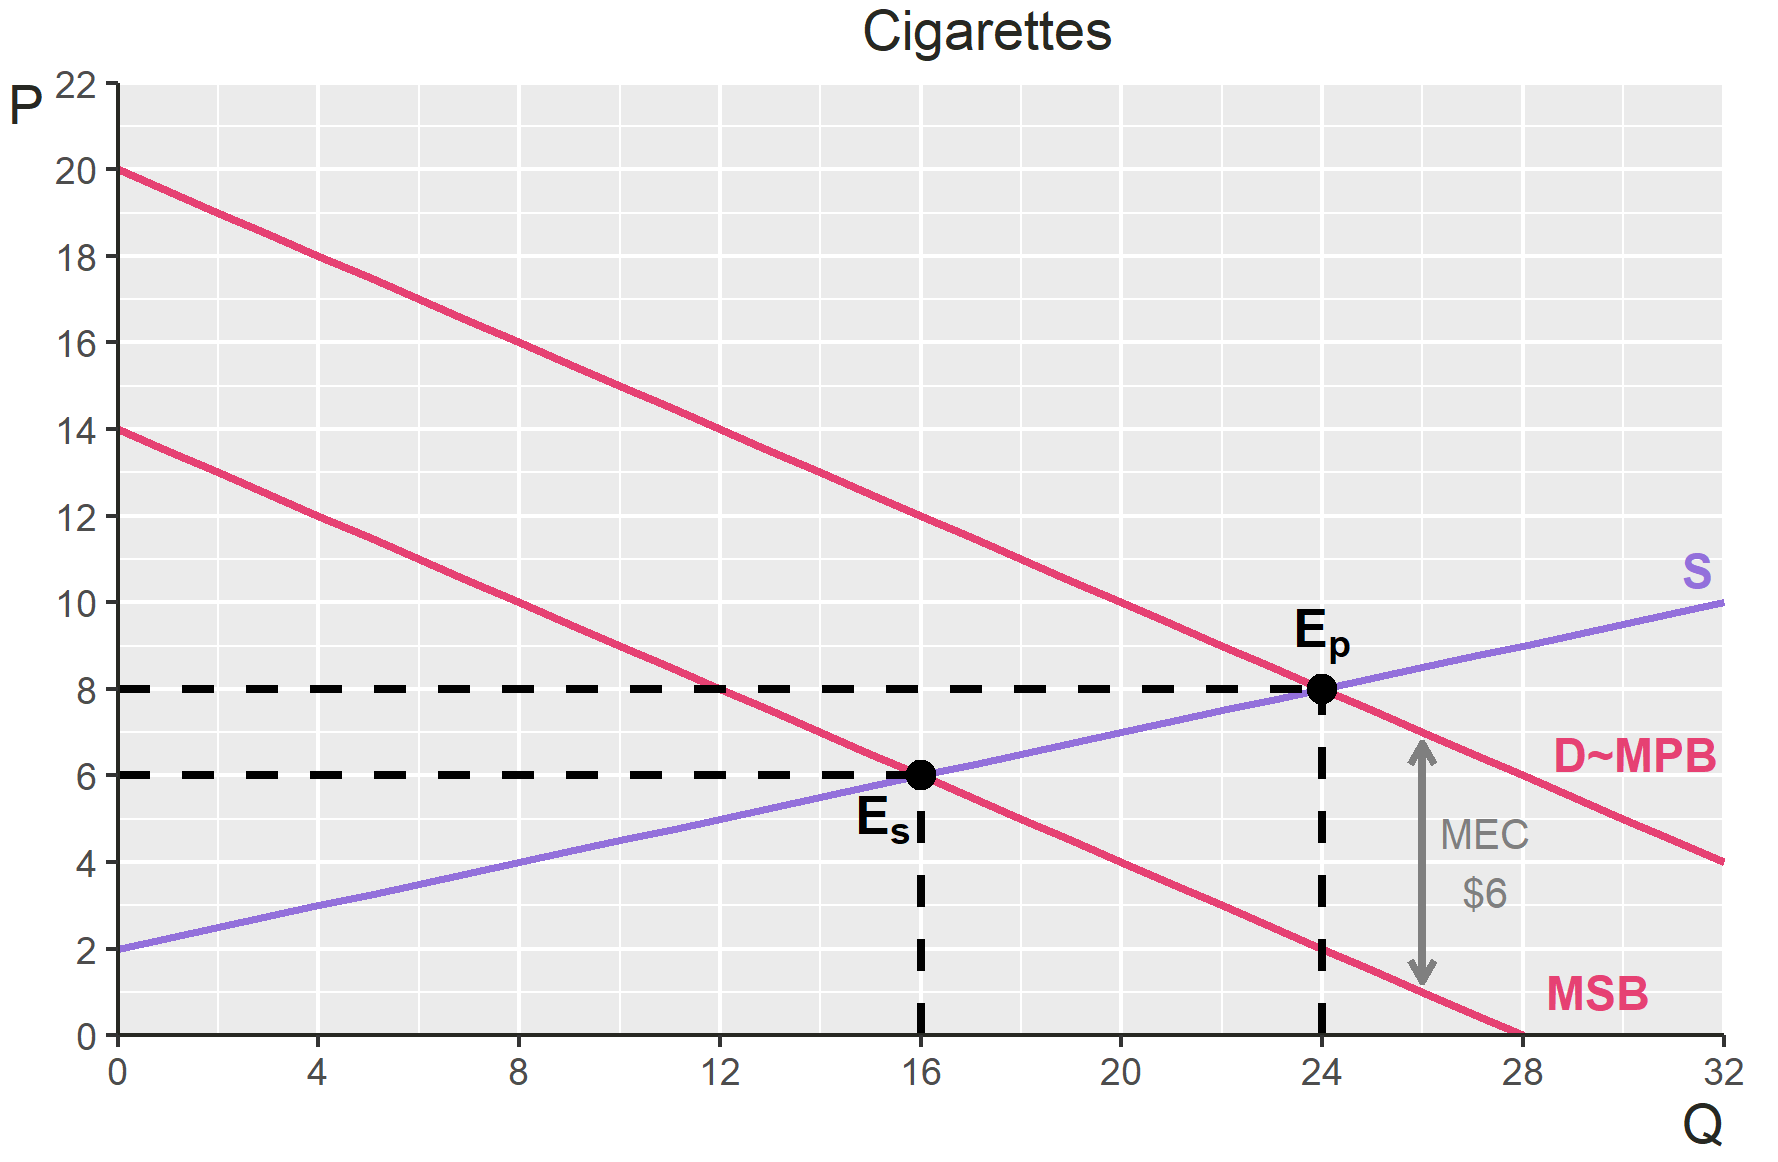
\includegraphics[width=8cm]{neg c ext base.png}
        \end{figure}
    \end{itemize}
\end{frame}

\begin{frame}{Negative Consumption Externality}
        \begin{figure}
            \centering
            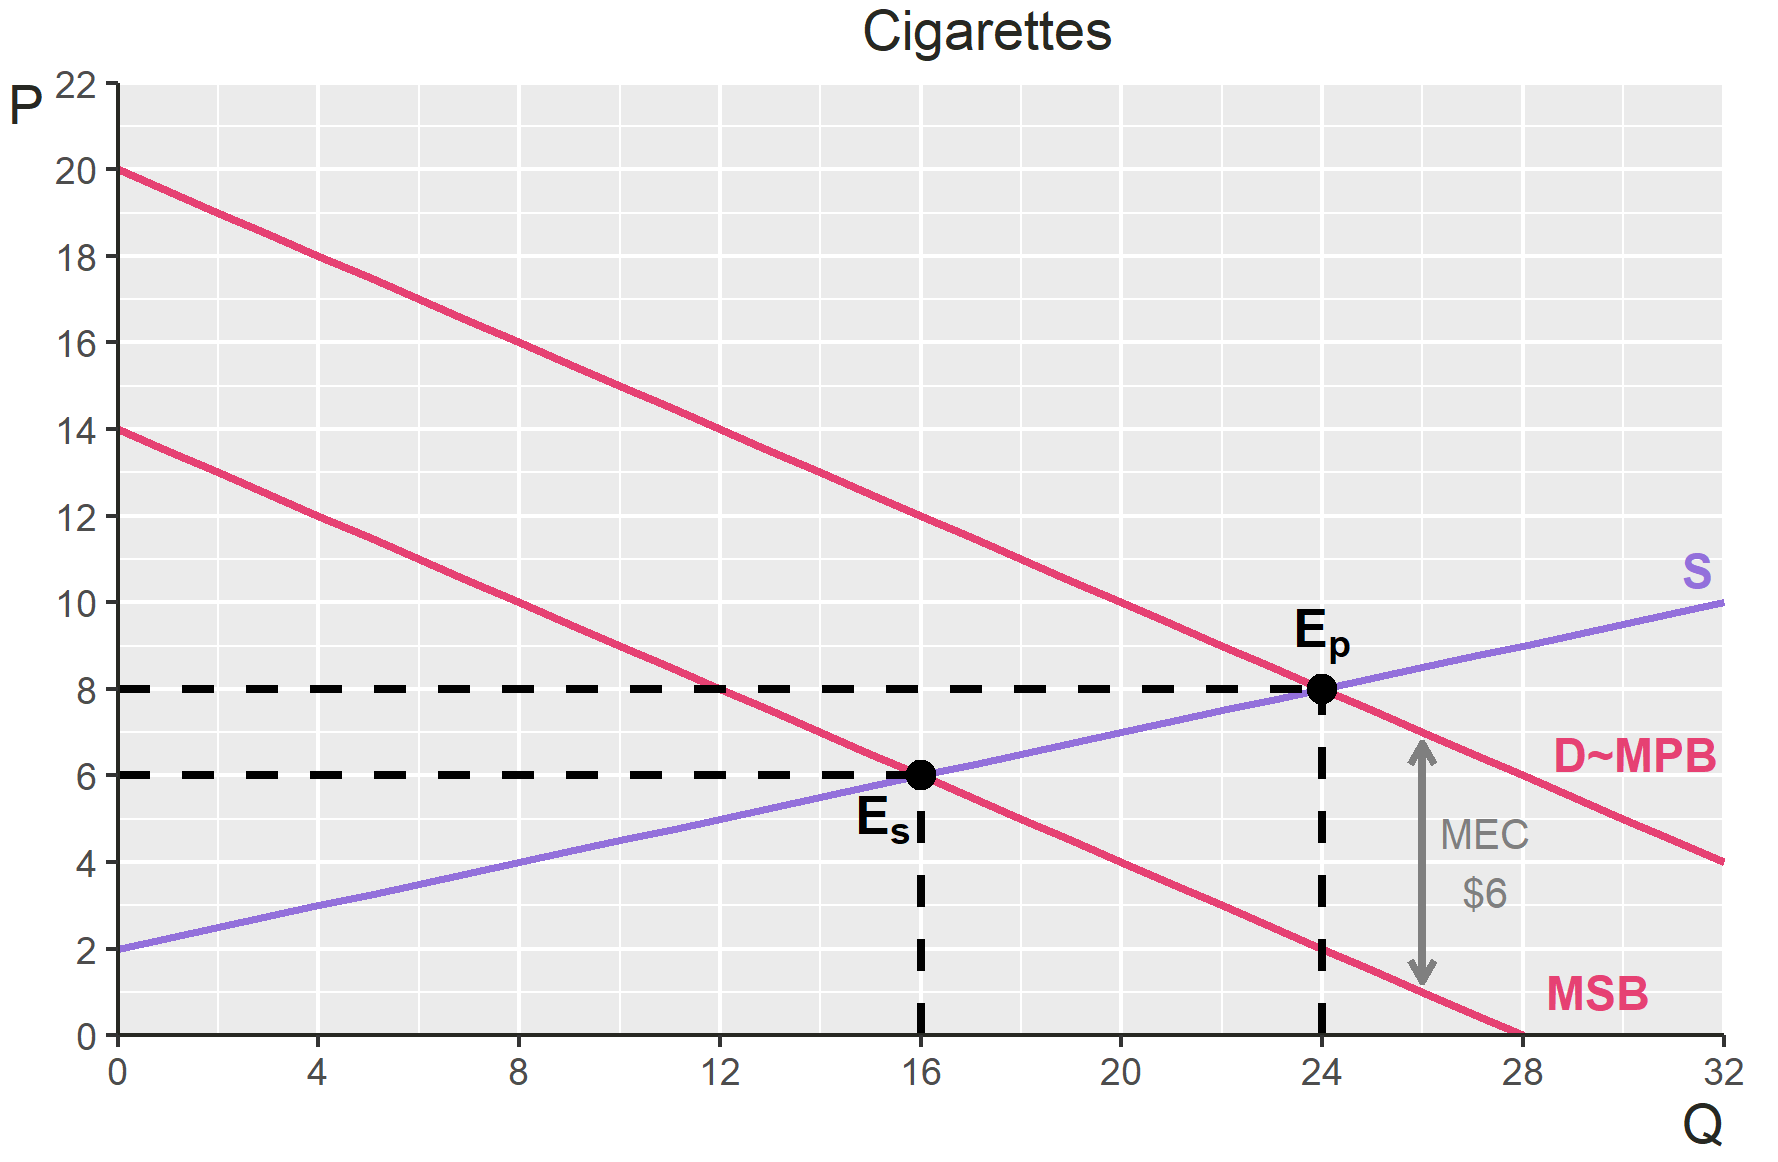
\includegraphics[width=8cm]{neg c ext base.png}
        \end{figure}
    \begin{itemize}[<+->]
    \vspace{-2mm}
        \item The social equilibrium, $E_{s}$, what society wants people to trade at, due to the spillover\footnote{\vspace{1mm}Another term for externality}
        \item The private equilibrium, $E_{p}$, is where we are at\vspace{1mm}
    \end{itemize}
\end{frame}

\begin{frame}{External Cost and External Benefit}
    \begin{itemize}[<+->]
        \item In order to measure the TS in the presence of an externality, we have to factor in the \textit{total} external benefit or cost, denoted EB (external benefit) or EC (external cost) 
        \item EB is counted \textit{positively} into TS, while EC is counted \textit{negatively} into TS
        \item EB and EC will always be parallelograms. The area of a parallelogram is $b\cdot h$
        \item EB is equal to the MEB times the amount traded, EC is equal to the MEC times the  amount traded
        \begin{align*}
            EB&=MEB\cdot Q^{*}\\
            EC&=MEC\cdot Q^{*}
        \end{align*}
    \end{itemize}
\end{frame}

\begin{frame}{Negative Consumption Externality}
    \begin{itemize}[<+->]
    \vspace{-1mm}
        \item What is EC in our cigarettes market, assuming the market is at private equilibrium?
        \begin{figure}
            \centering
            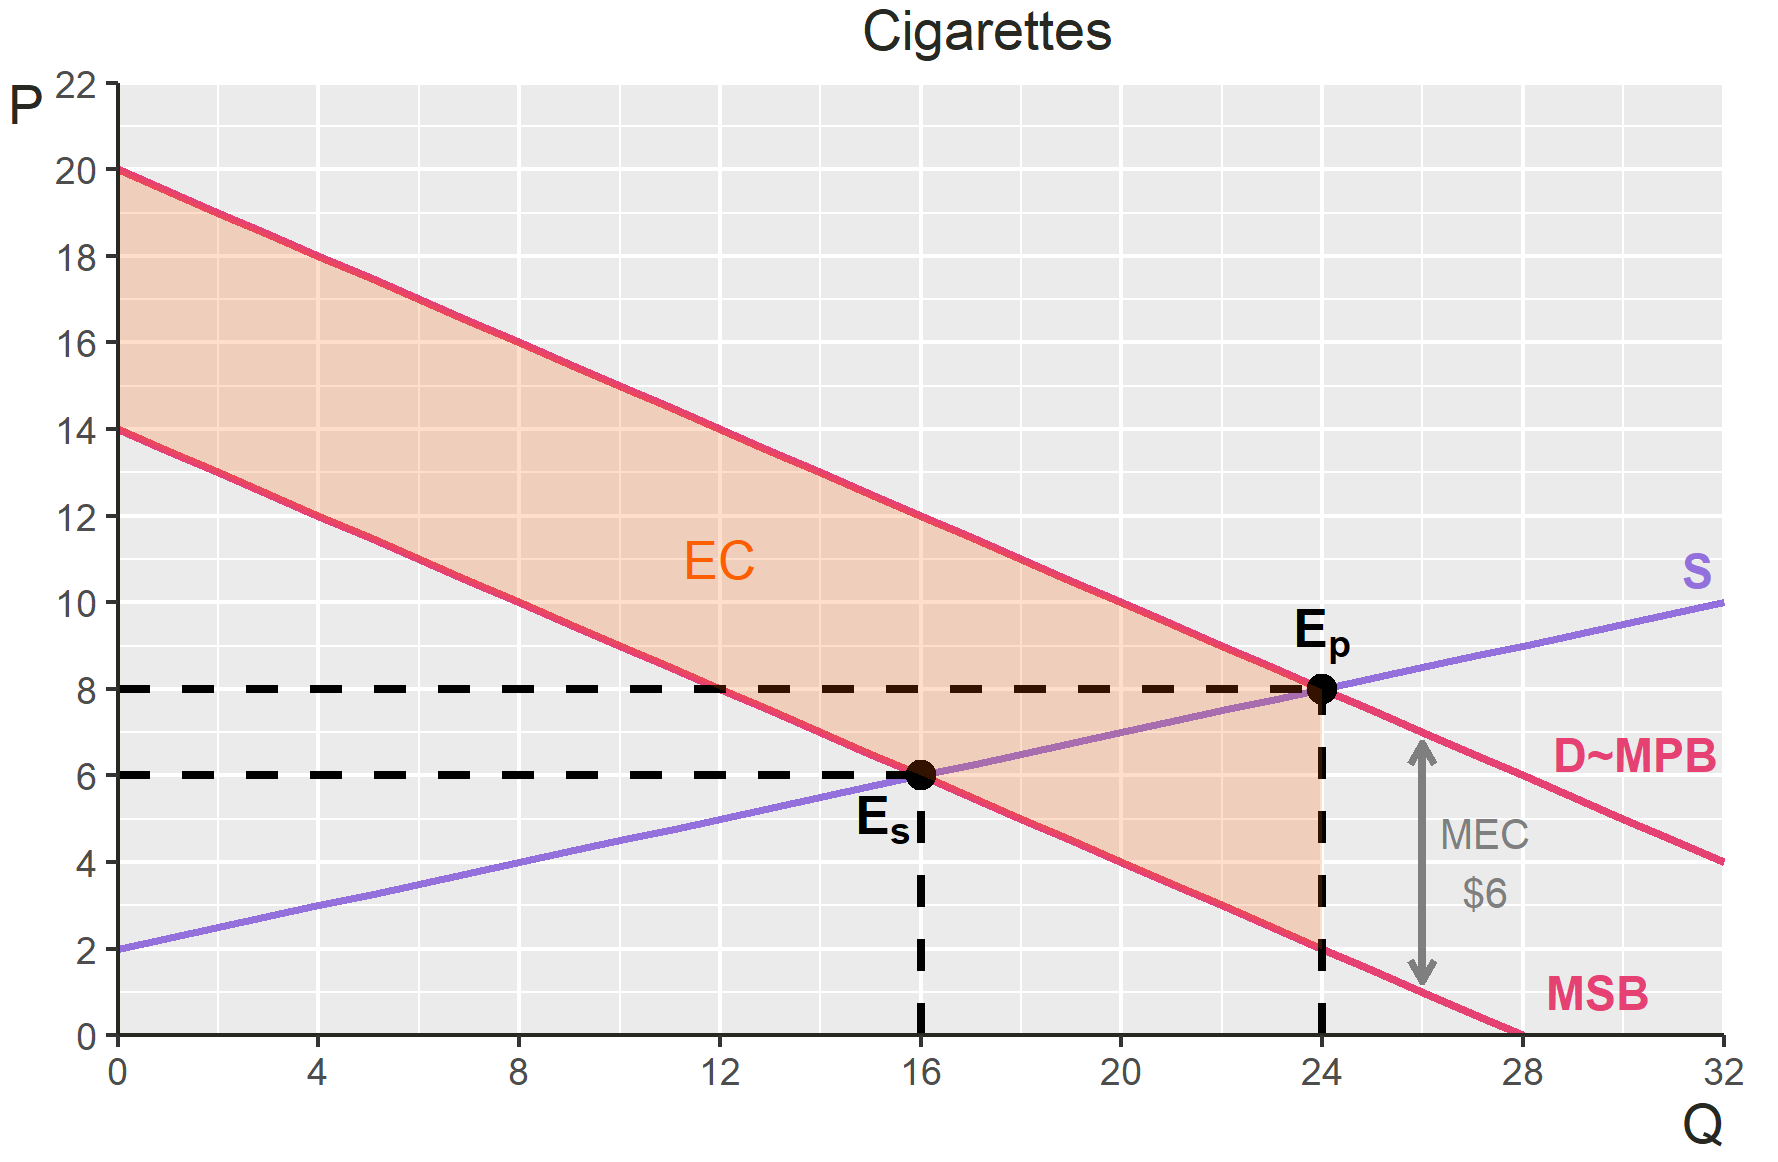
\includegraphics[width=7cm]{neg c ext ec.png}
        \end{figure}
        $$EC=b\cdot h=24(20-14)=(24)(6)=144$$
    \end{itemize}
\end{frame}

\begin{frame}{Negative Consumption Externality}
    \begin{itemize}[<+->]
    \vspace{-1mm}
        \item What is CS+PS in our cigarettes market, assuming the market is at private equilibrium?
        \begin{figure}
            \centering
            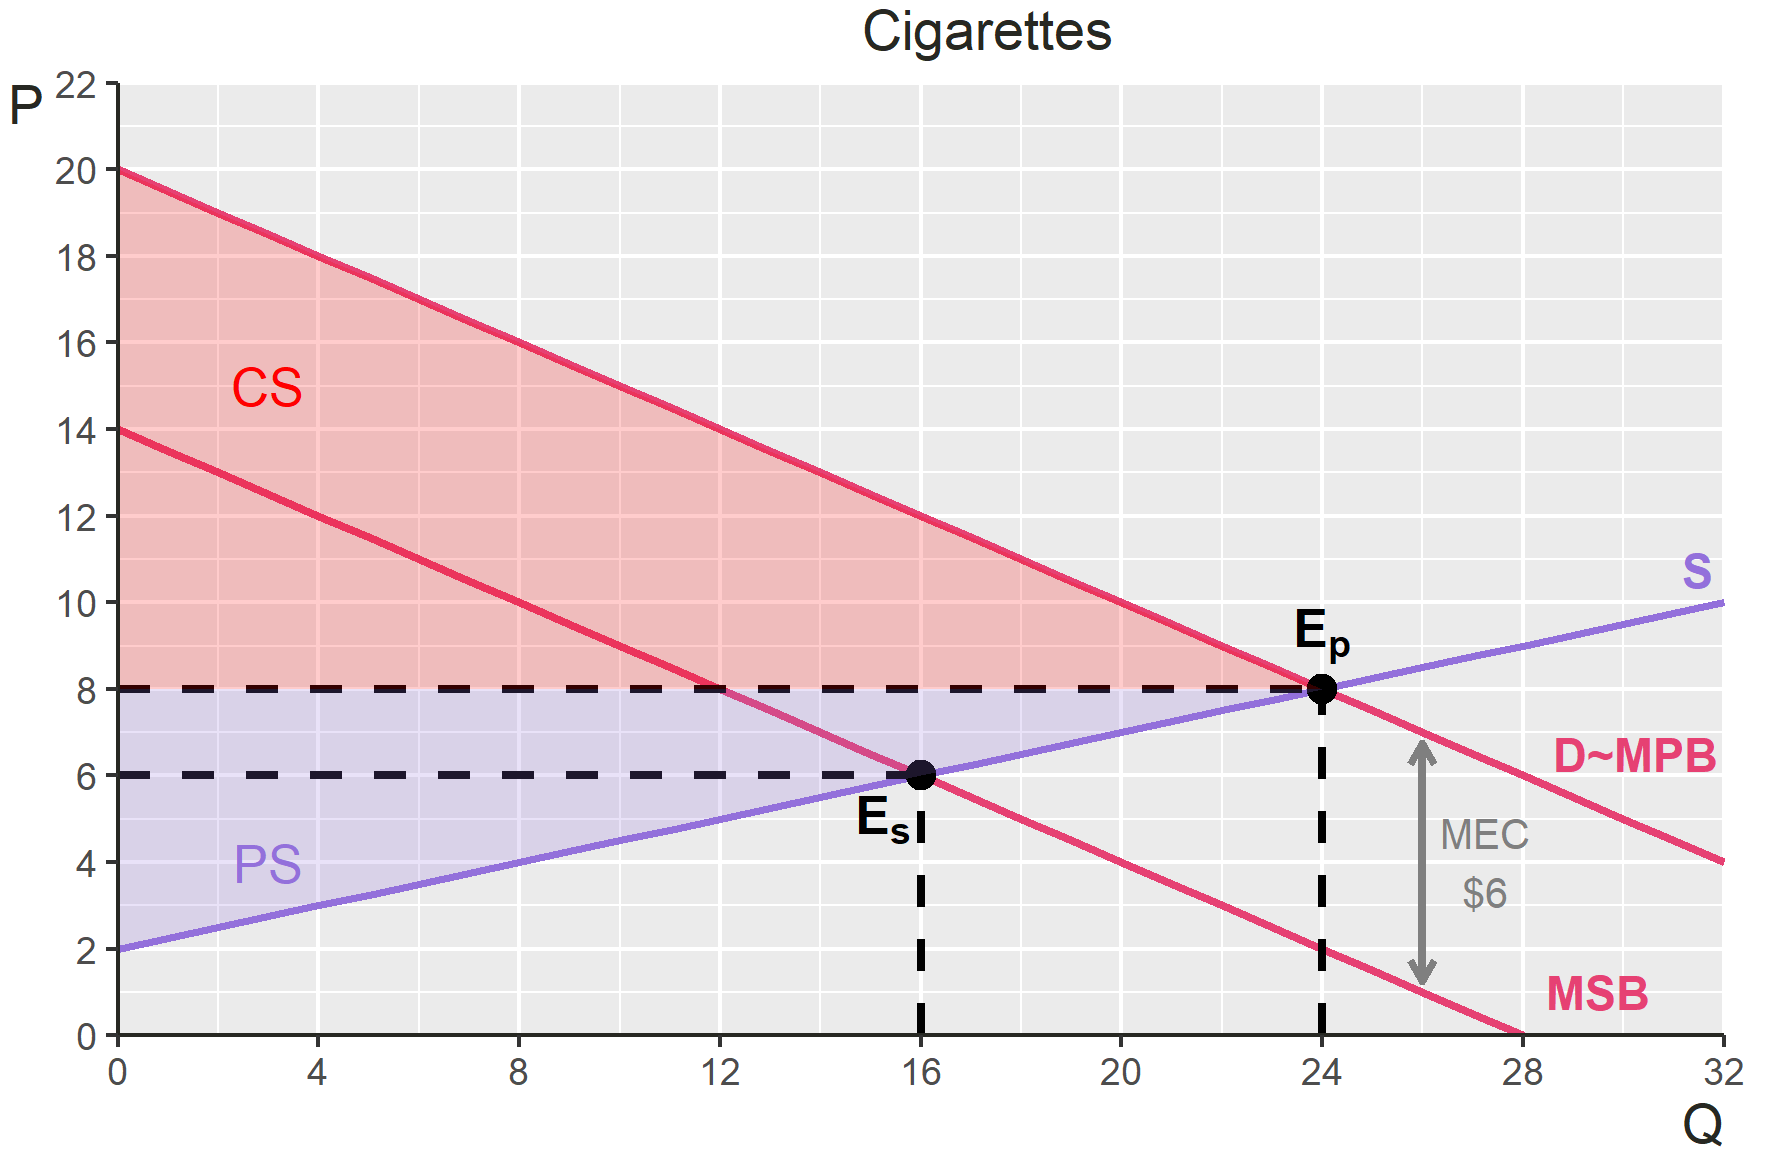
\includegraphics[width=7cm]{neg c ext csps.png}
        \end{figure}
        \vspace{-1mm}
        \begin{align*}
            CS&=\frac{1}{2}(24)(20-8)=144\\
            PS&=\frac{1}{2}(24)(8-2)=72
        \end{align*}
    \end{itemize}
\end{frame}

\begin{frame}{Negative Consumption Externality}
    \begin{itemize}[<+->]
    \vspace{-1mm}
        \item Thus, total surplus is in private equilibrium is 
        $$TS=CS+PS-EC=144+72-144=72$$
        \item Can we do better?
    \end{itemize}
\end{frame}

\begin{frame}{How do we Correct for Externalities?}
    \begin{itemize}[<+->]
        \item It costs society when people smoke. How do we induce them not to smoke?
        \item I.e., how do we make them \textit{internalize} the externality?
        \begin{itemize}
            \item Tax them!
        \end{itemize}
        \item How much do we tax them?
        \item The exact amount of the marginal external cost!
    \end{itemize}
\end{frame}

\begin{frame}{Negative Consumption Externality}
    \begin{itemize}[<+->]
        \item Under a $\$6$ tax, demand just \textit{becomes} MSB:
        \begin{figure}
            \centering
            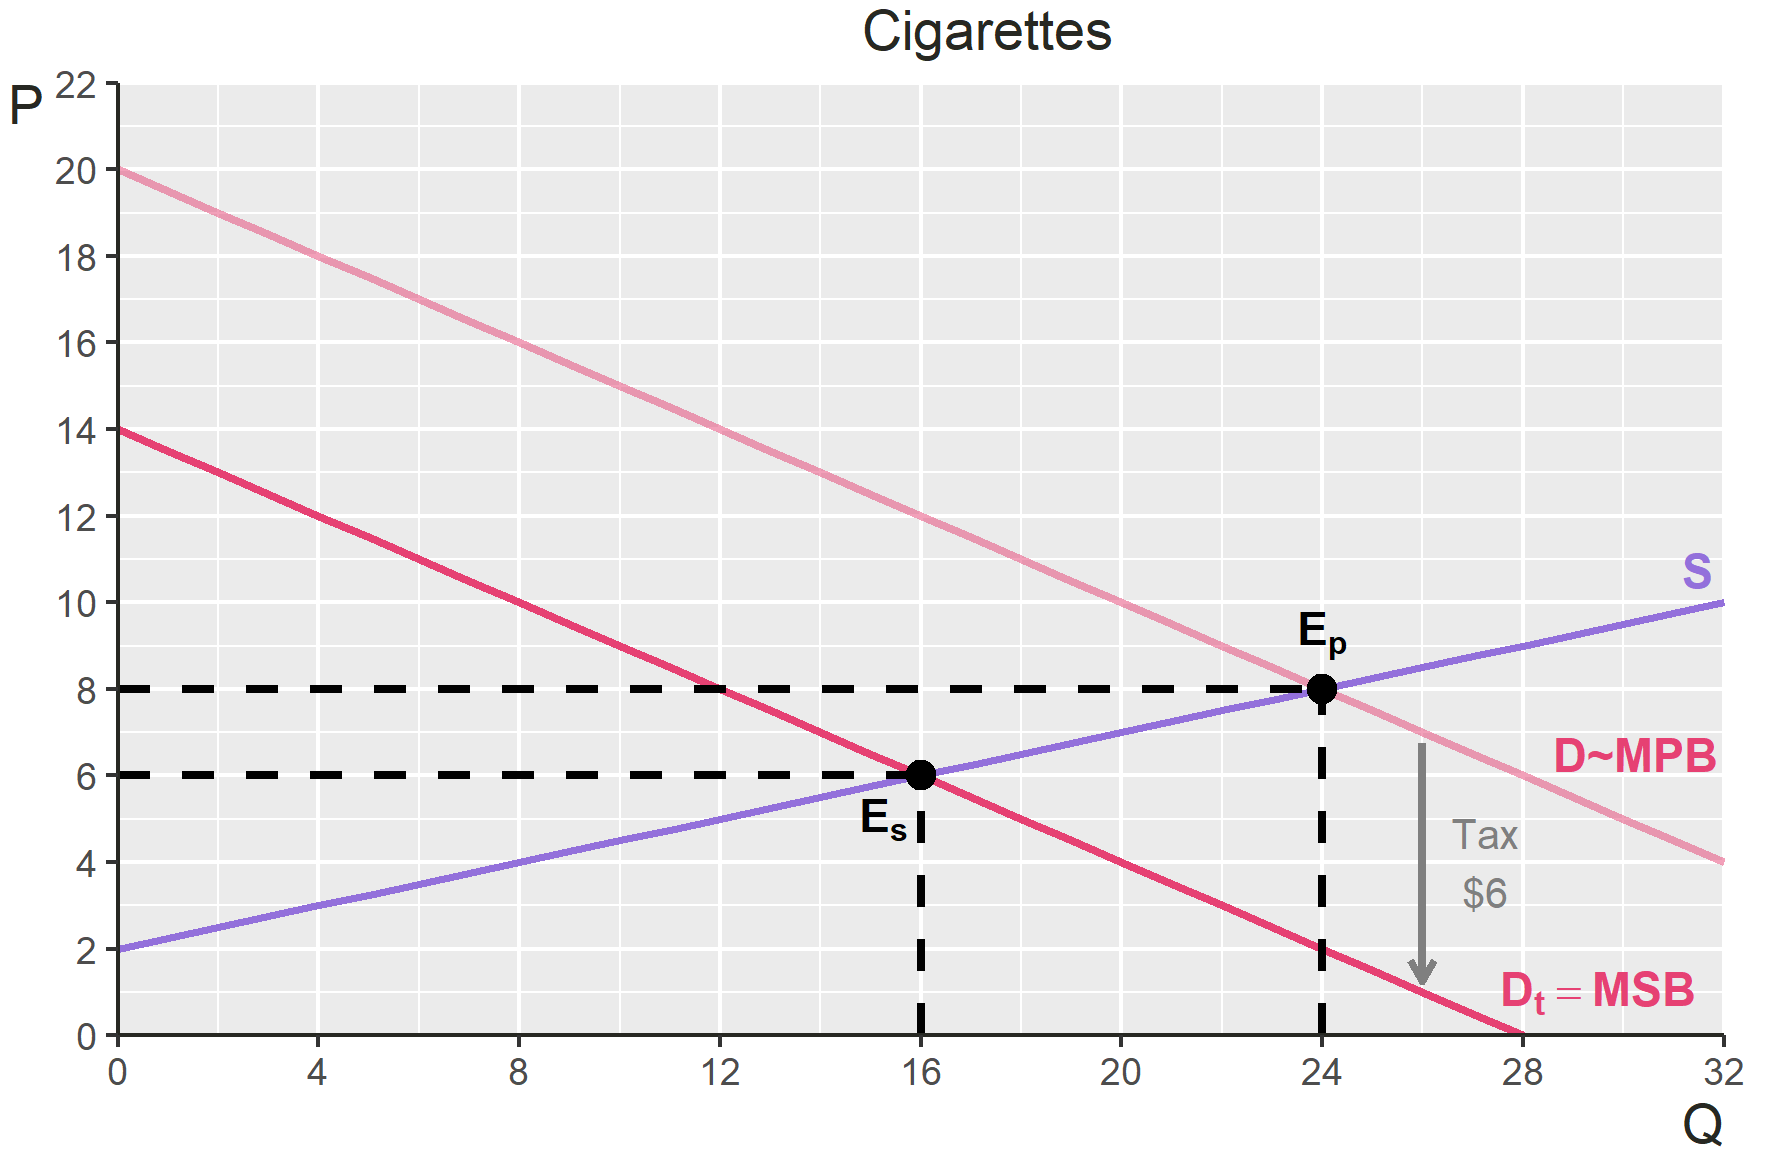
\includegraphics[width=7cm]{cnext tax base.png}
        \end{figure}
    \end{itemize}
\end{frame}

\begin{frame}{Negative Consumption Externality}
    \begin{itemize}[<+->]
        \item CS and PS are as expected:
        \begin{figure}
            \centering
            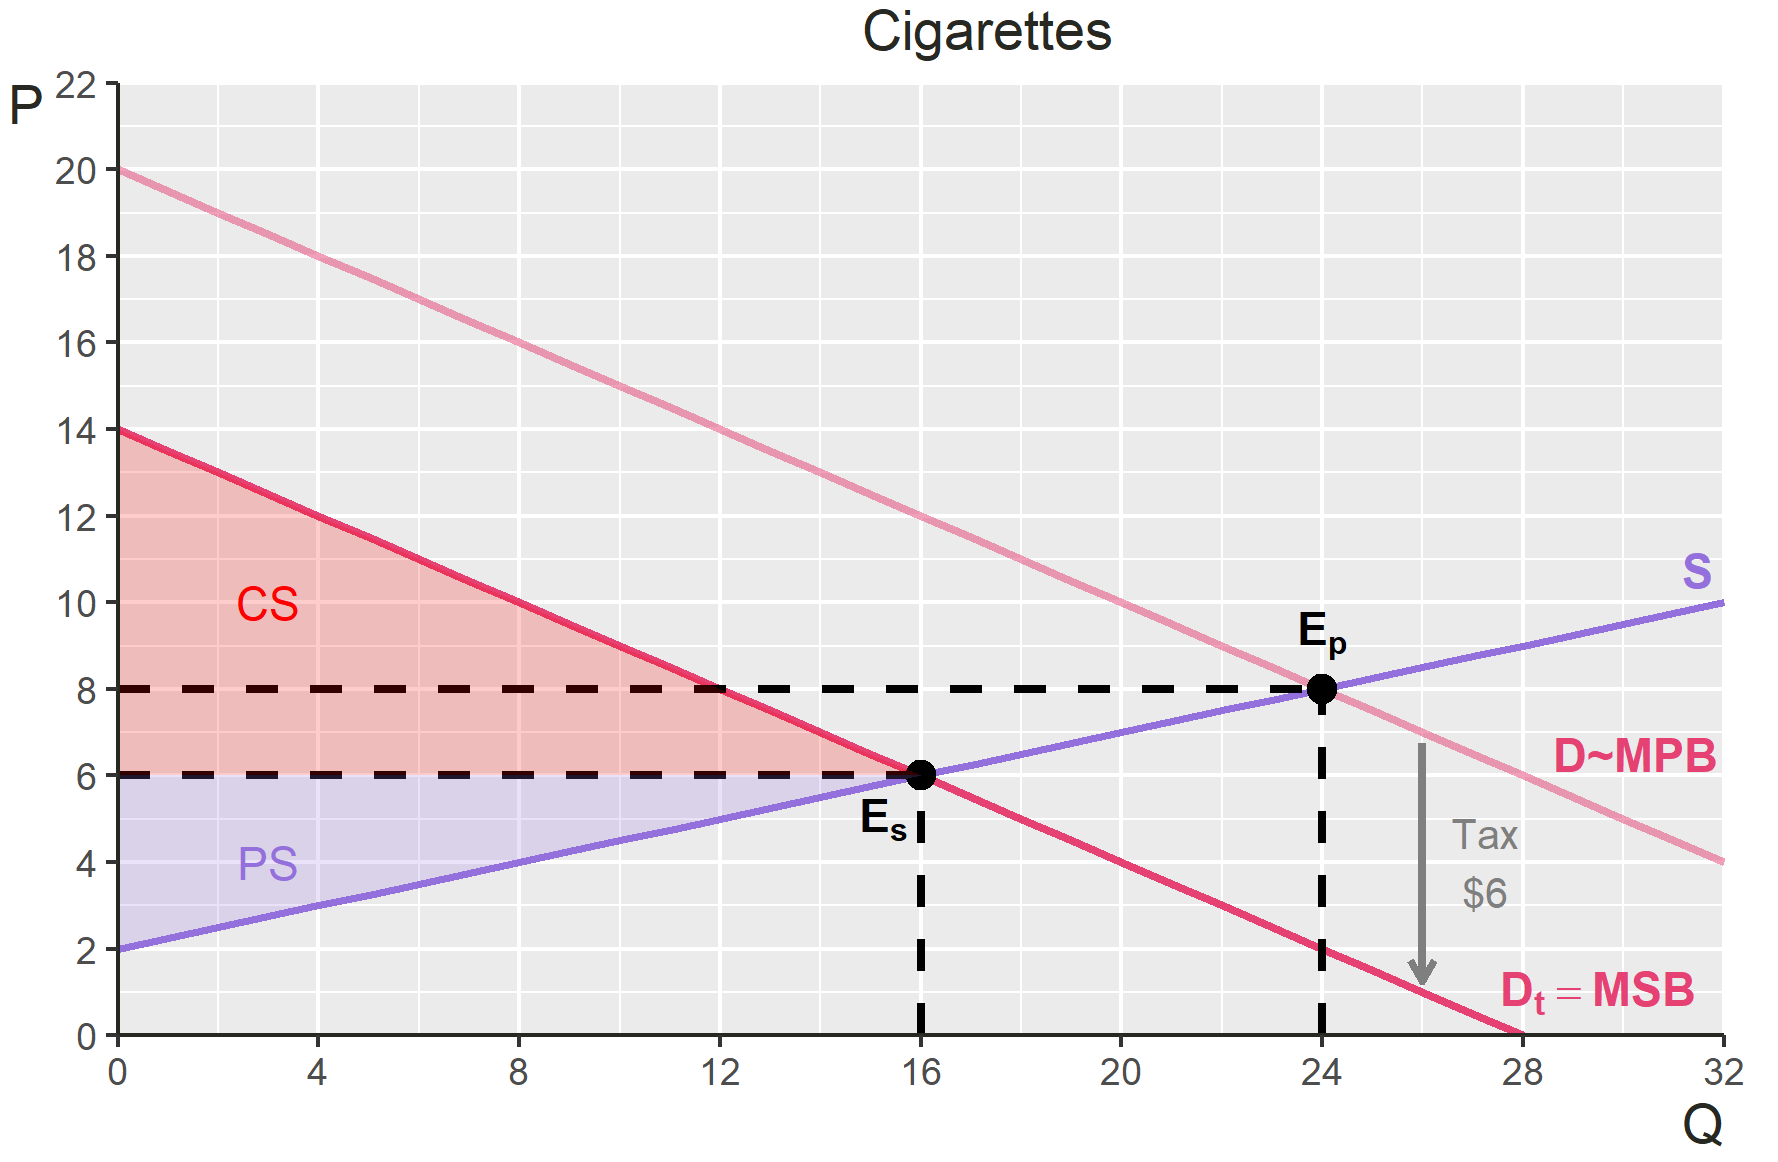
\includegraphics[width=7cm]{cnext tax csps.png}
        \end{figure}
        \begin{align*}
            CS&=\frac{1}{2}(16)(14-6)=64\\
            PS&=\frac{1}{2}(16)(6-2)=32
        \end{align*}
    \end{itemize}
\end{frame}

\begin{frame}{Negative Consumption Externality}
    \begin{itemize}[<+->]
        \item The EC is now given by
        \begin{figure}
            \centering
            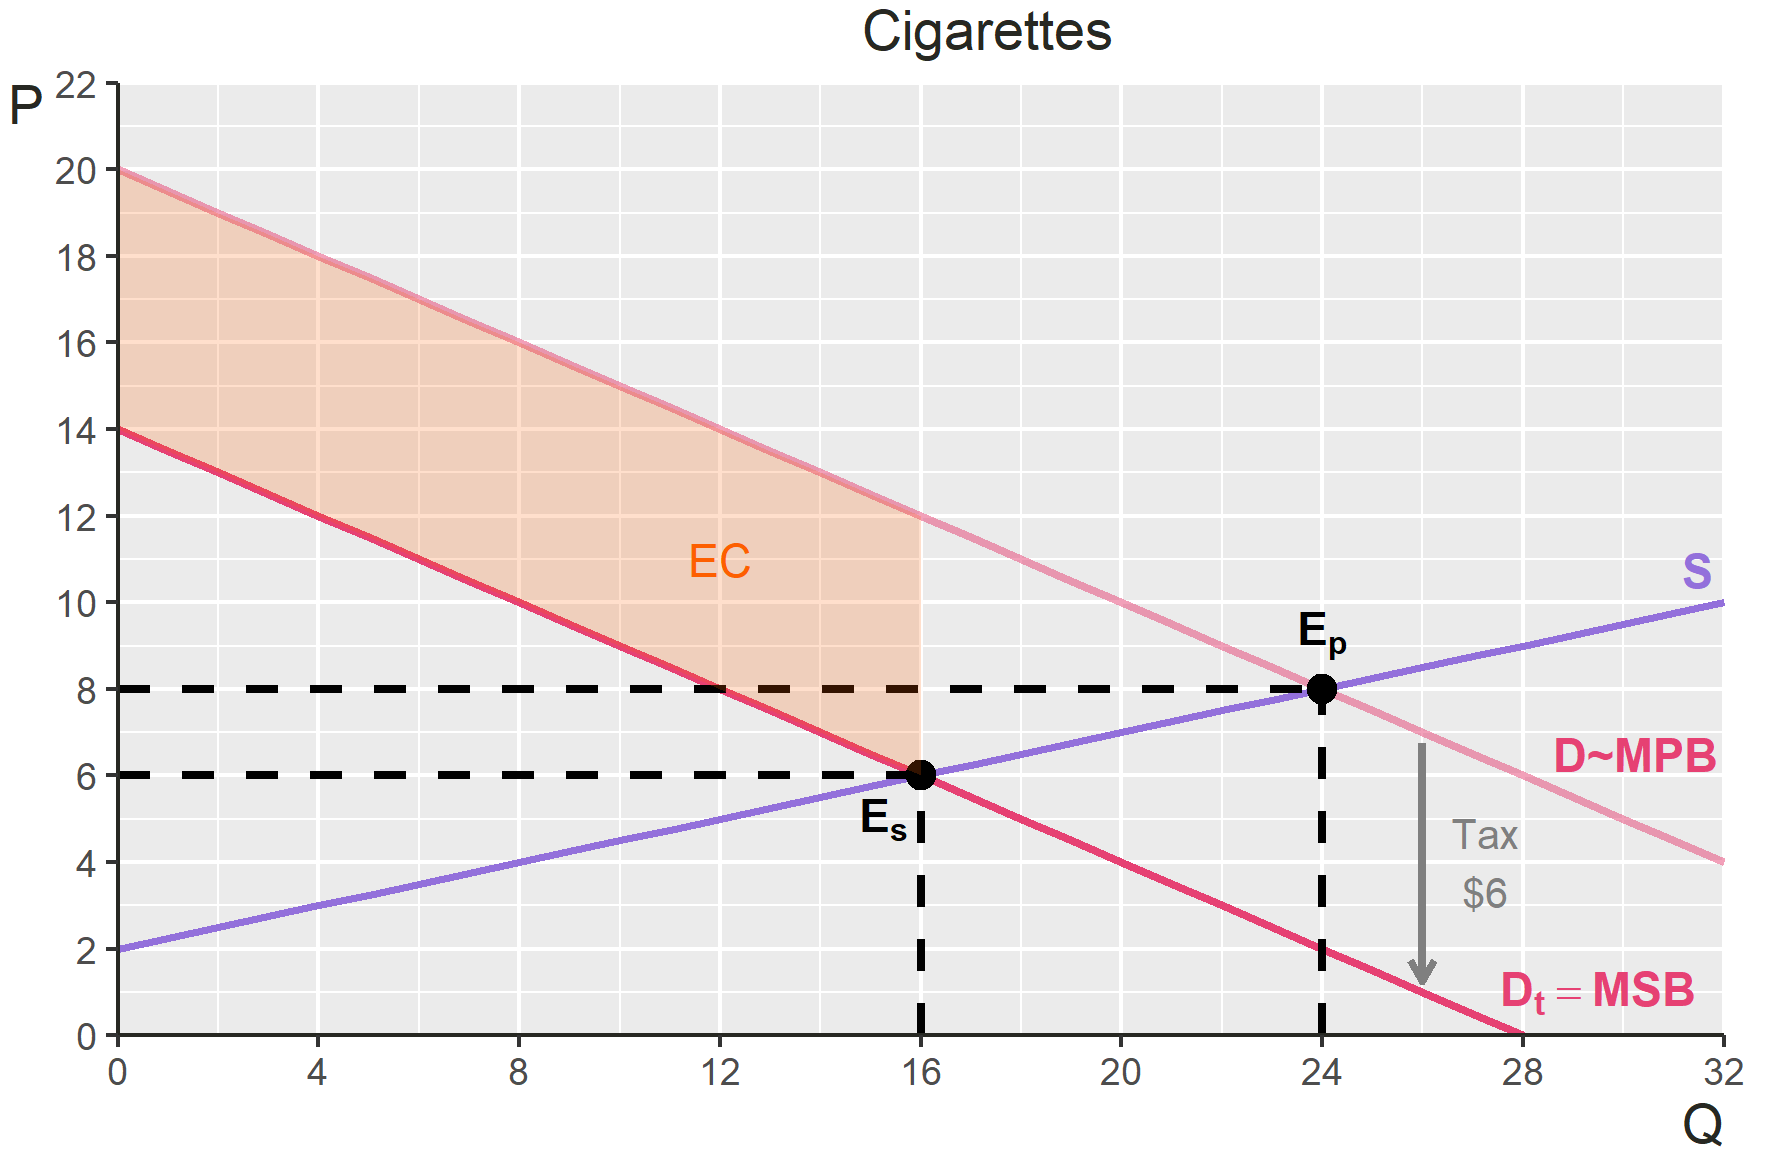
\includegraphics[width=7cm]{cnext tax ec.png}
        \end{figure}
        $$EC=(16)(6)=96$$
    \end{itemize}
\end{frame}

\begin{frame}{Negative Consumption Externality}
    \begin{itemize}[<+->]
        \item And now, we have some GR
        \begin{figure}
            \centering
            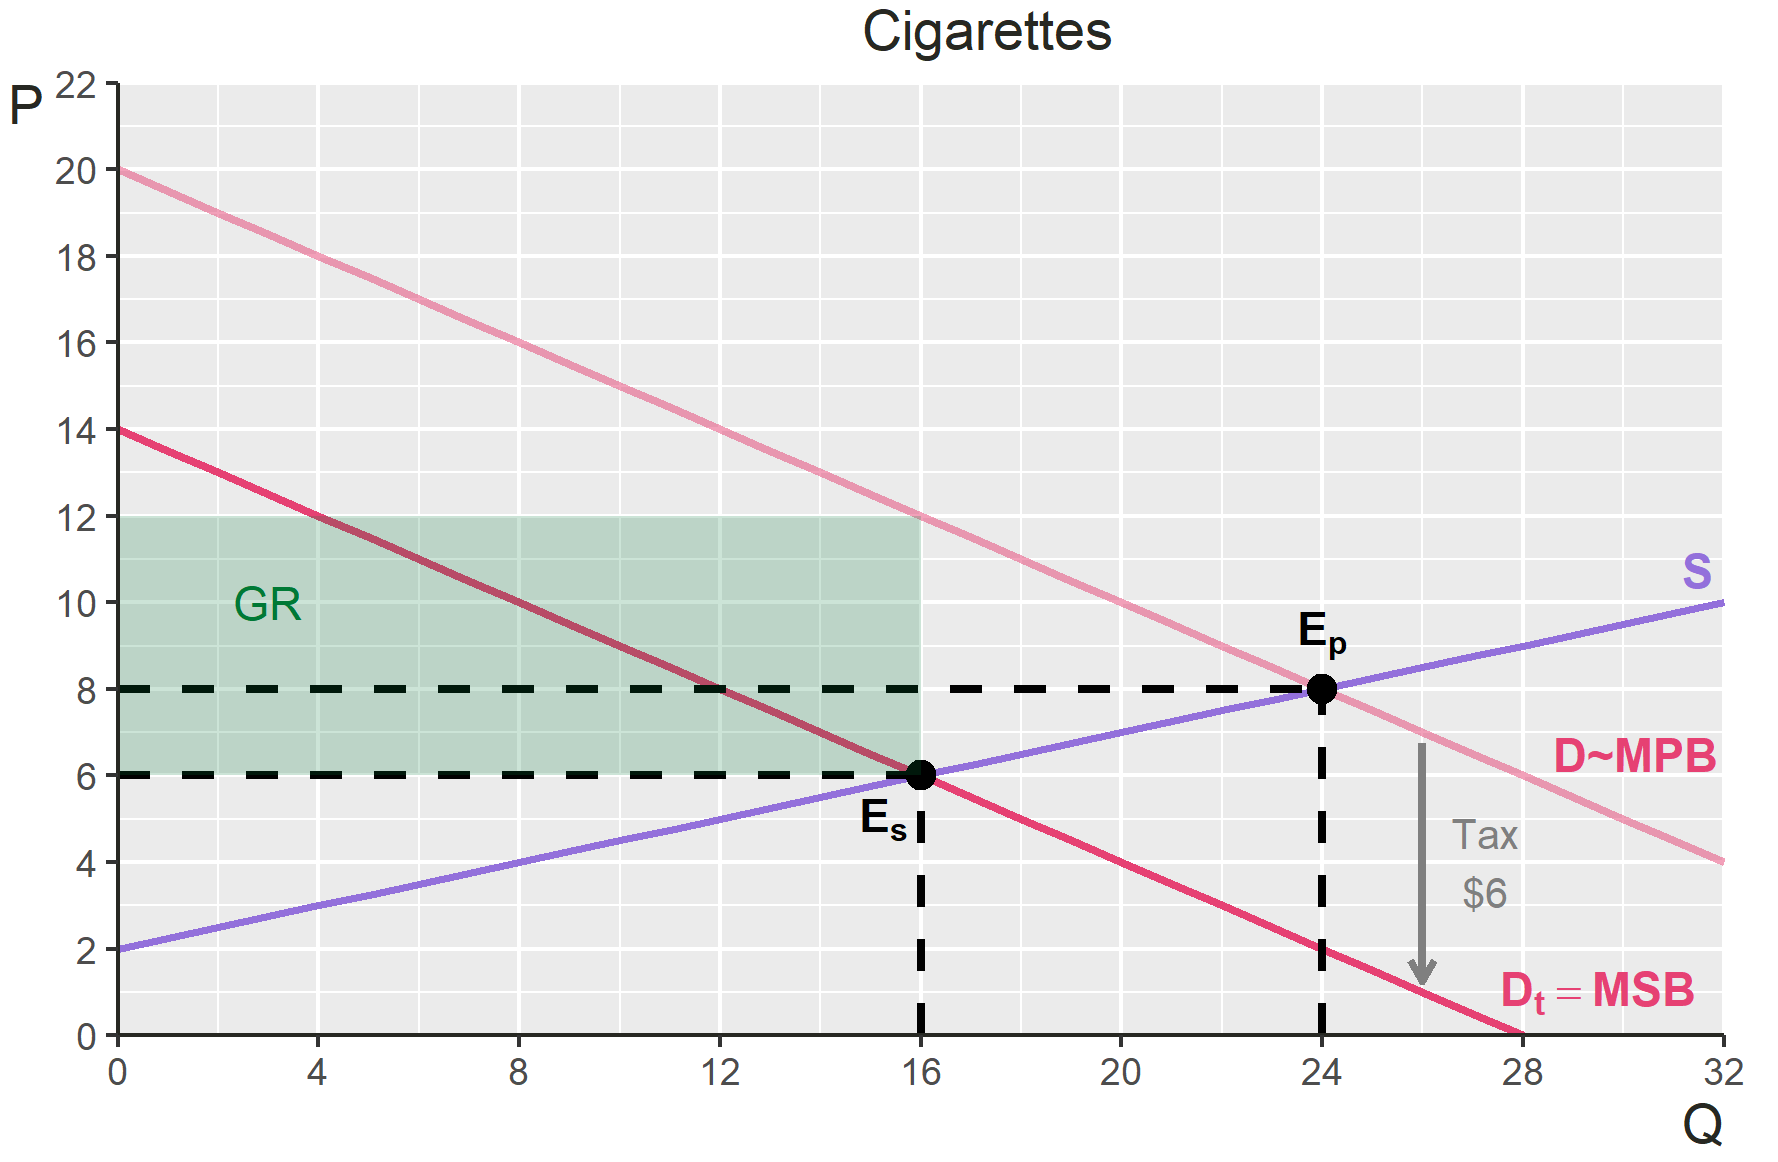
\includegraphics[width=7cm]{cnext tax gr.png}
        \end{figure}
        $$GR=(16)(6)=96$$
    \end{itemize}
\end{frame}

\begin{frame}{Negative Consumption Externality}
    \begin{itemize}[<+->]
        \item What happens?
        \begin{itemize}
            \item GR exactly cancels out the new EC!
        \end{itemize}
        \item What is the new TS?
        \begin{itemize}
            \item The new TS is given by 
            $$TS=CS+PS-EC+GR=64+32-96+96=96$$
        \end{itemize}
        \item This beats the 72 from before, and is also in fact the maximum possible TS in this example
        \item Therefore, taxation actually \textit{induced} efficiency 
        \begin{itemize}
            \item This is the key lesson: a tax will fix an negative externality 
        \end{itemize}
    \end{itemize}
\end{frame}

\begin{frame}{Negative Consumption Externality}
    \begin{itemize}[<+->]
        \item Therefore, DWL before the tax is given by 
        \begin{figure}
            \centering
            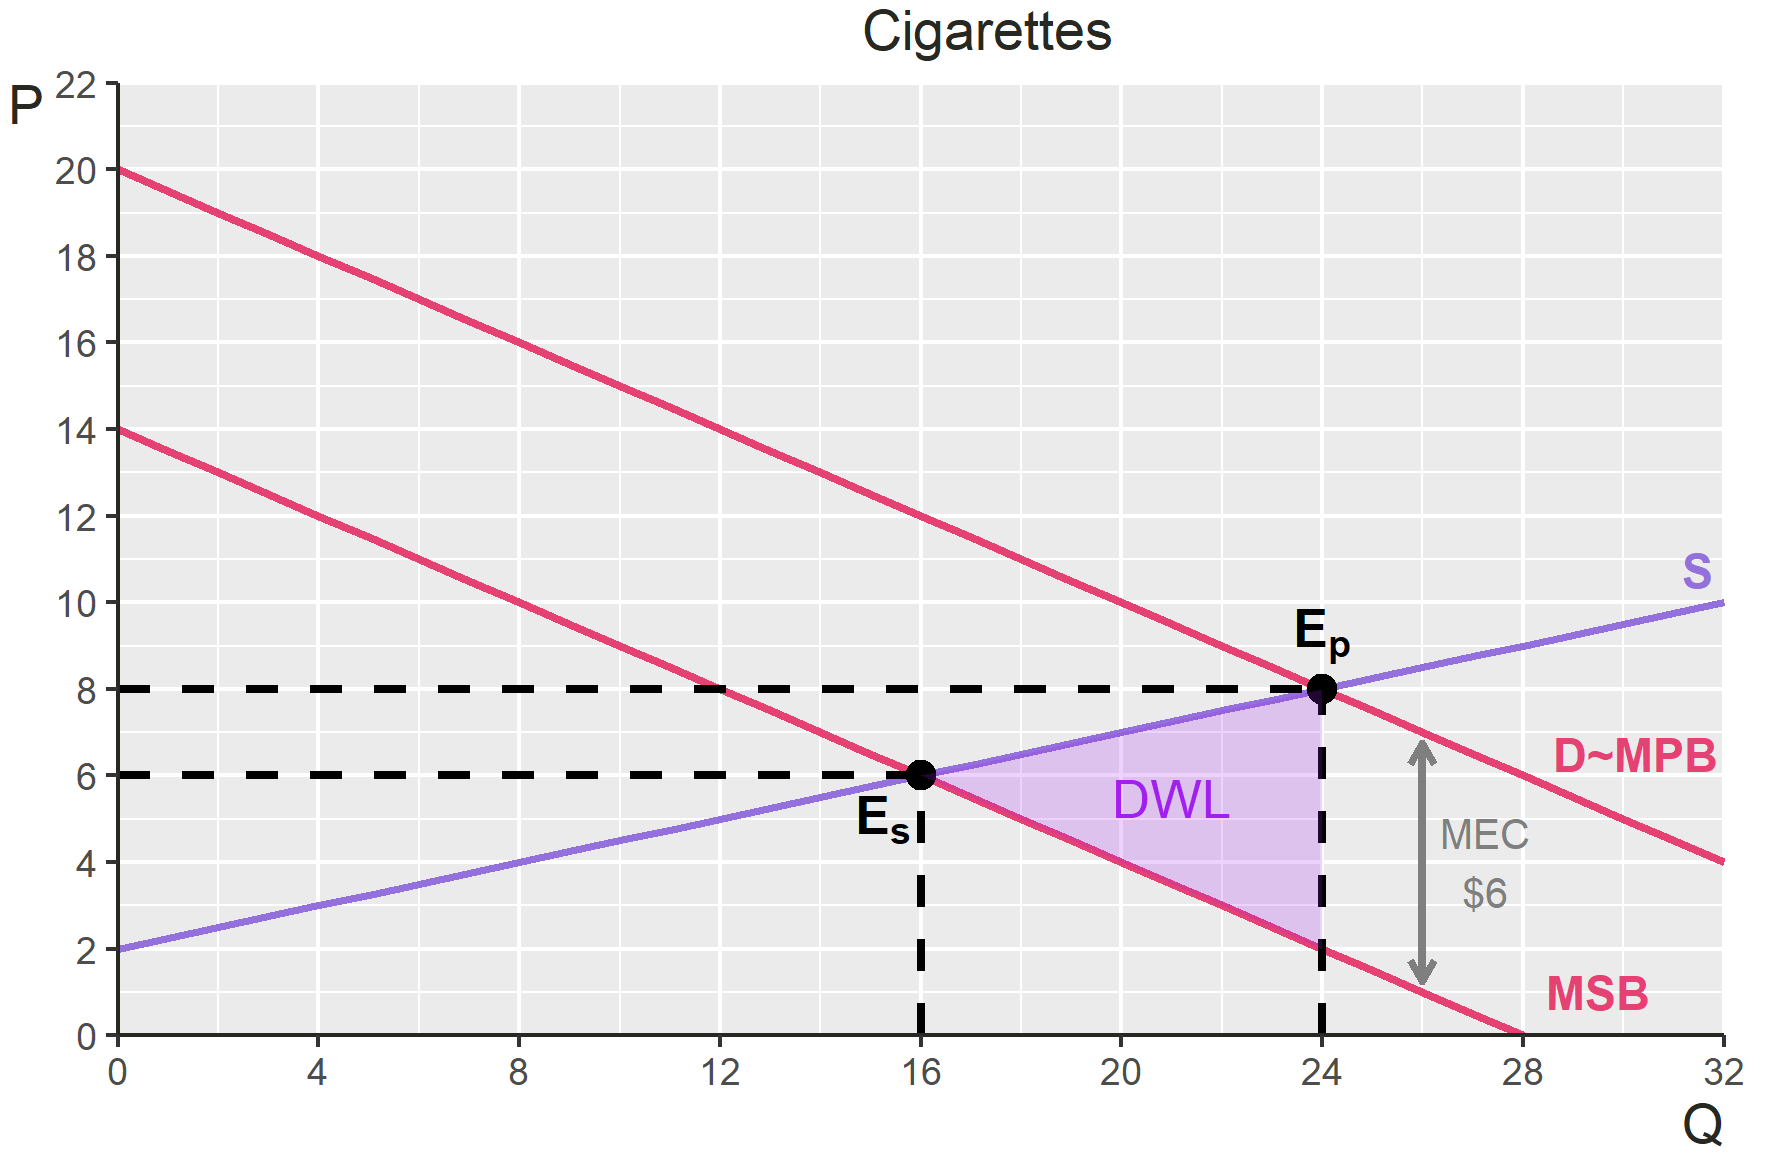
\includegraphics[width=7cm]{neg c ext dwl.png}
        \end{figure}
        $$DWL=\frac{1}{2}(24-16)(8-2)=24$$
    \end{itemize}
\end{frame}


%%%%%EX 2
\subsection*{Ex 2}

\begin{frame}{Negative Production Externality}
    \begin{itemize}[<+->]
        \item Suppose there is an MEC of $\$40$ for every barrel of oil made
        \begin{figure}
            \centering
            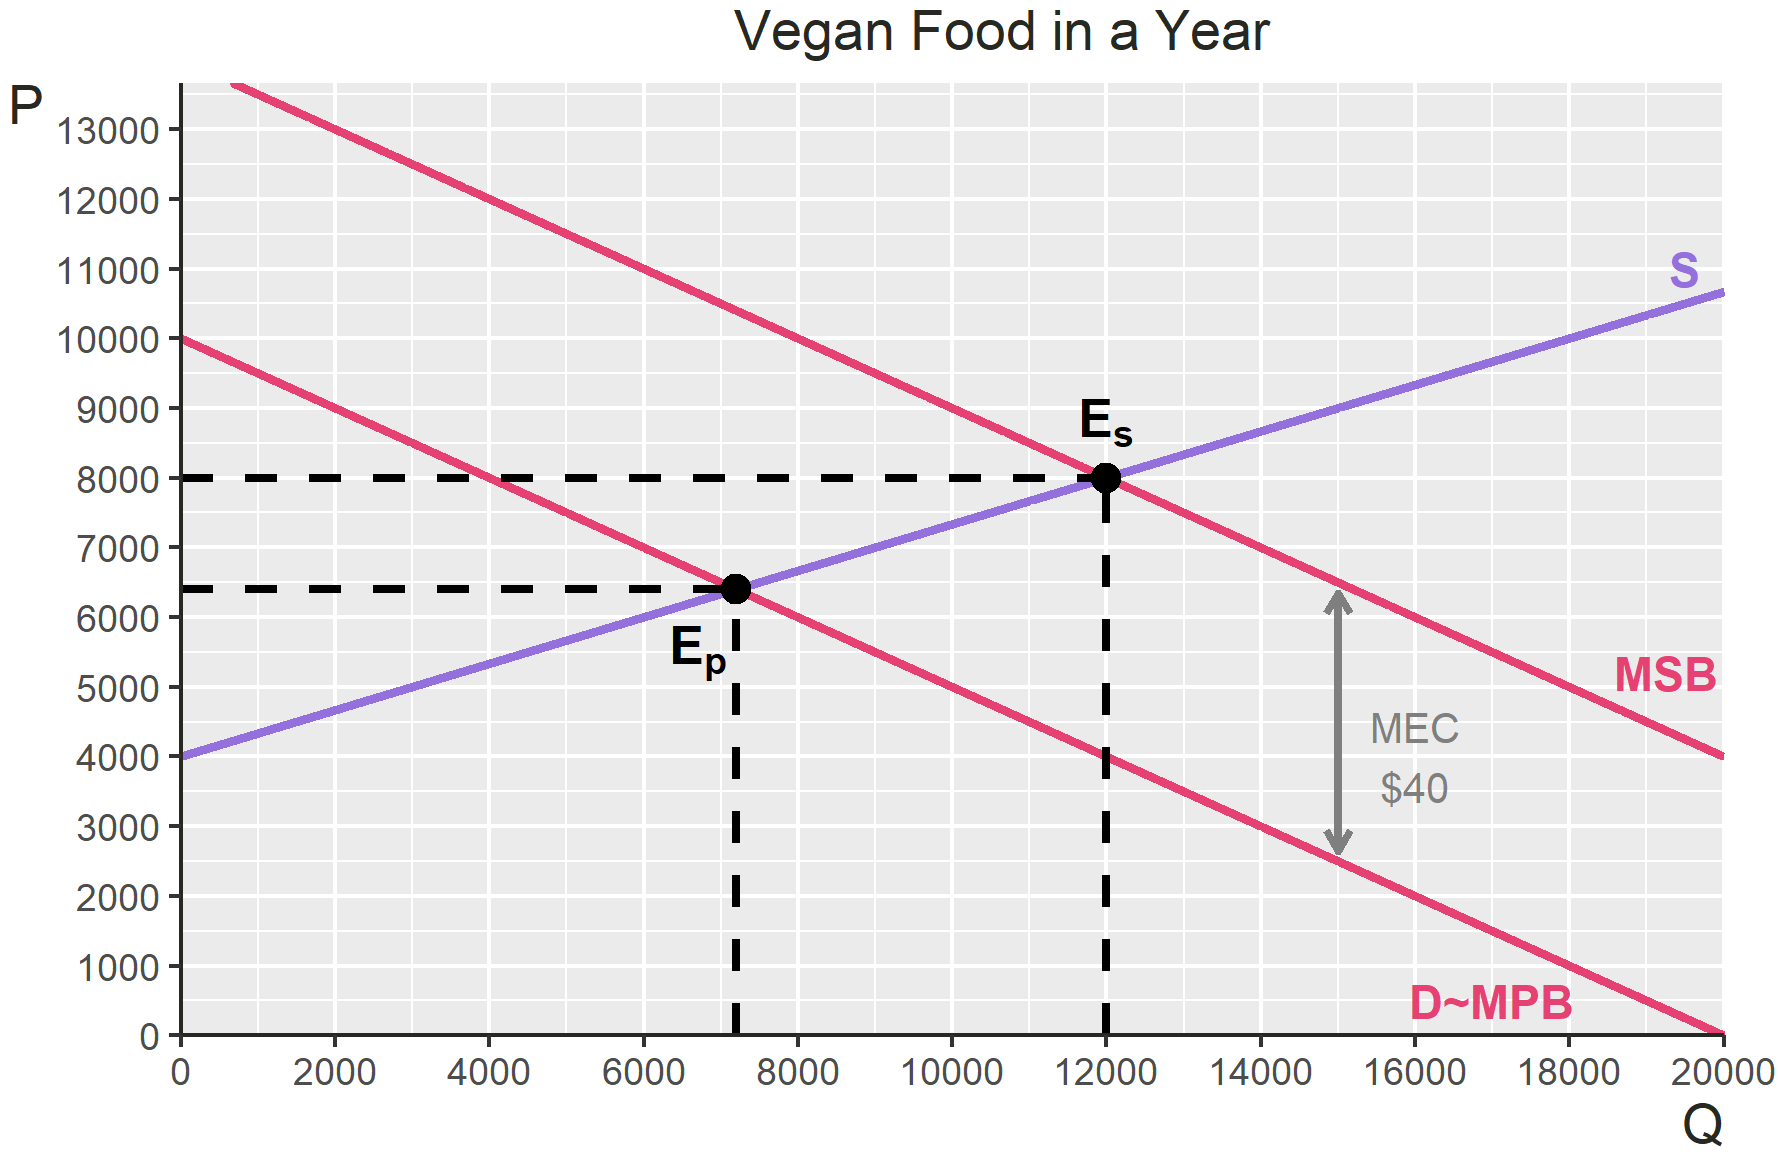
\includegraphics[width=8cm]{pnext base.png}
        \end{figure}
        \item $E_{s}$ what society wants people to trade at, while the $E_{p}$ is where we are at
    \end{itemize}
\end{frame}

\begin{frame}{Negative Production Externality}
    \begin{itemize}[<+->]
    \vspace{-1mm}
        \item What is EC?
        \begin{figure}
            \centering
            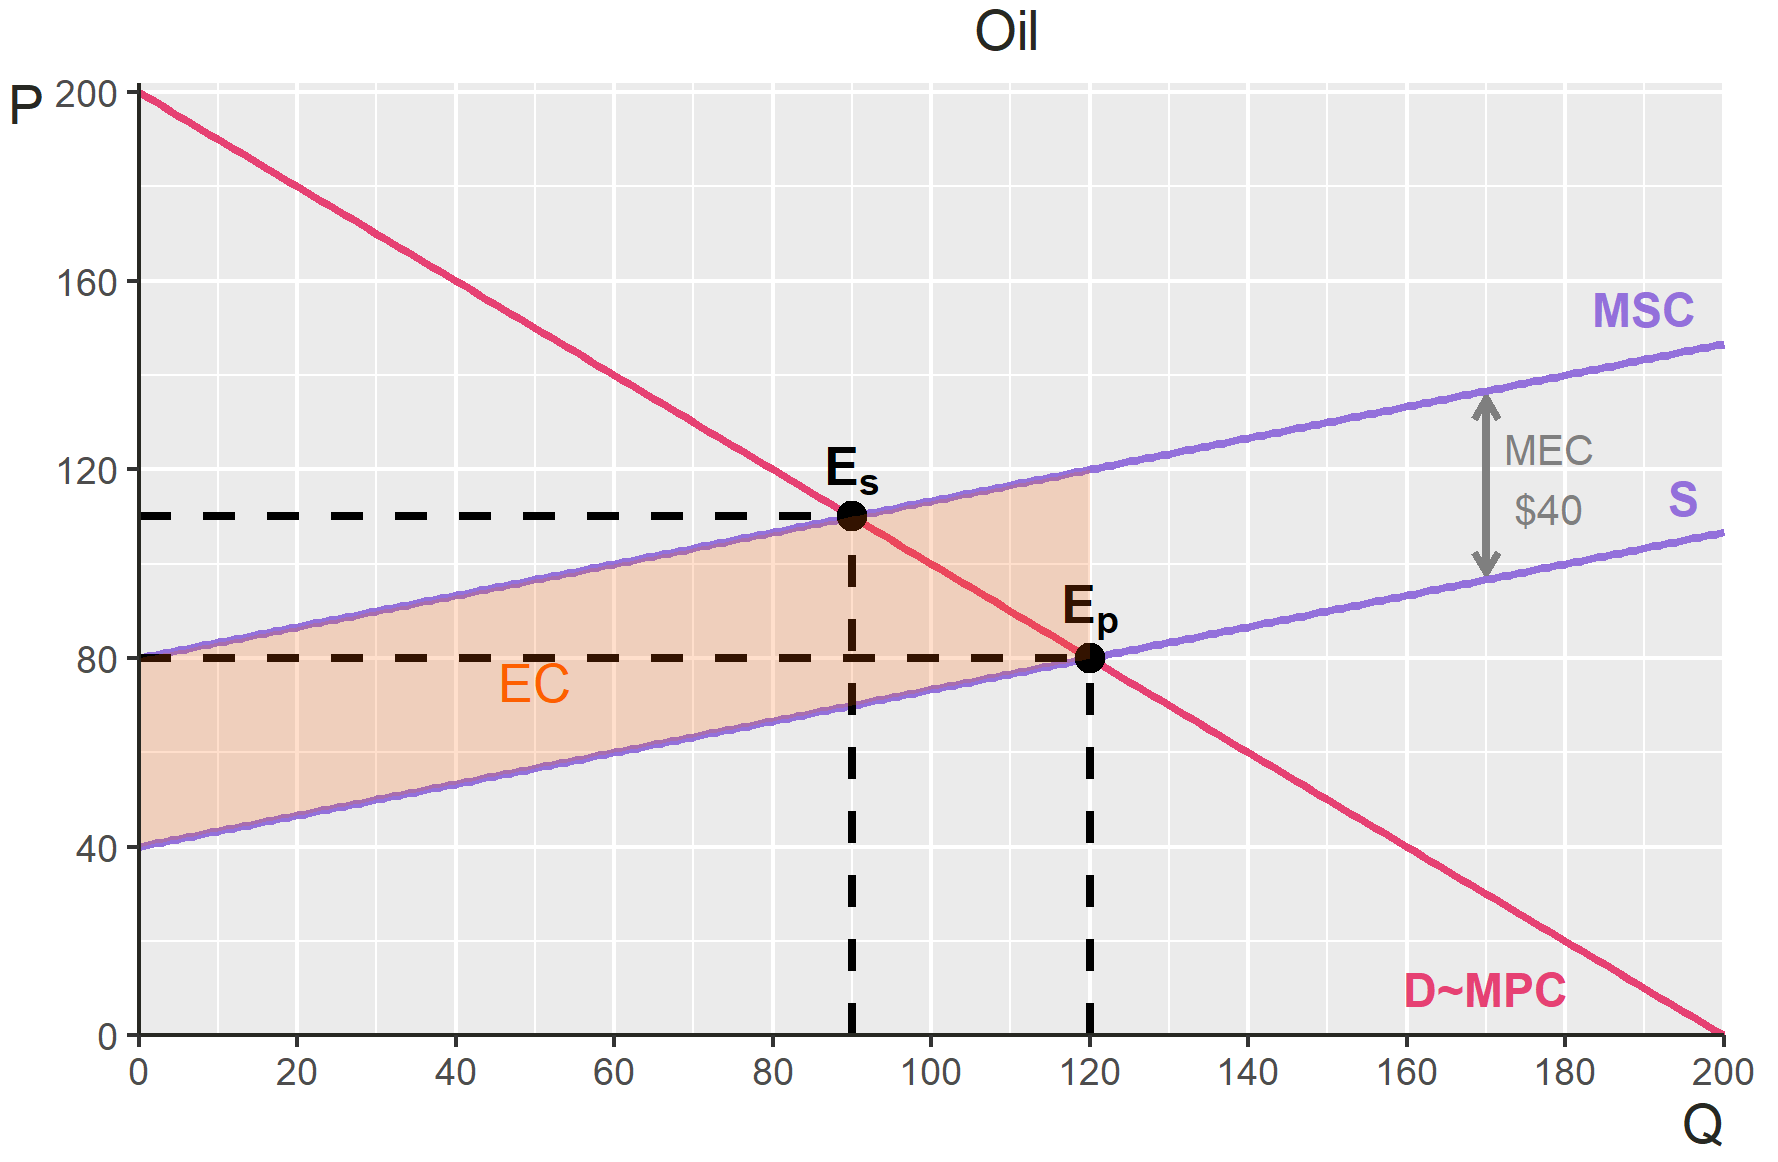
\includegraphics[width=7cm]{pnextec.png}
        \end{figure}
        $$EC=b\cdot h=120(80-40)=4800$$
    \end{itemize}
\end{frame}

\begin{frame}{Negative Production Externality}
    \begin{itemize}[<+->]
        \item Suppose we implement a $\$40$/unit producer tax to try to diminish production, so that our new supply line is just equal to $MSC$:
        \begin{figure}
            \centering
            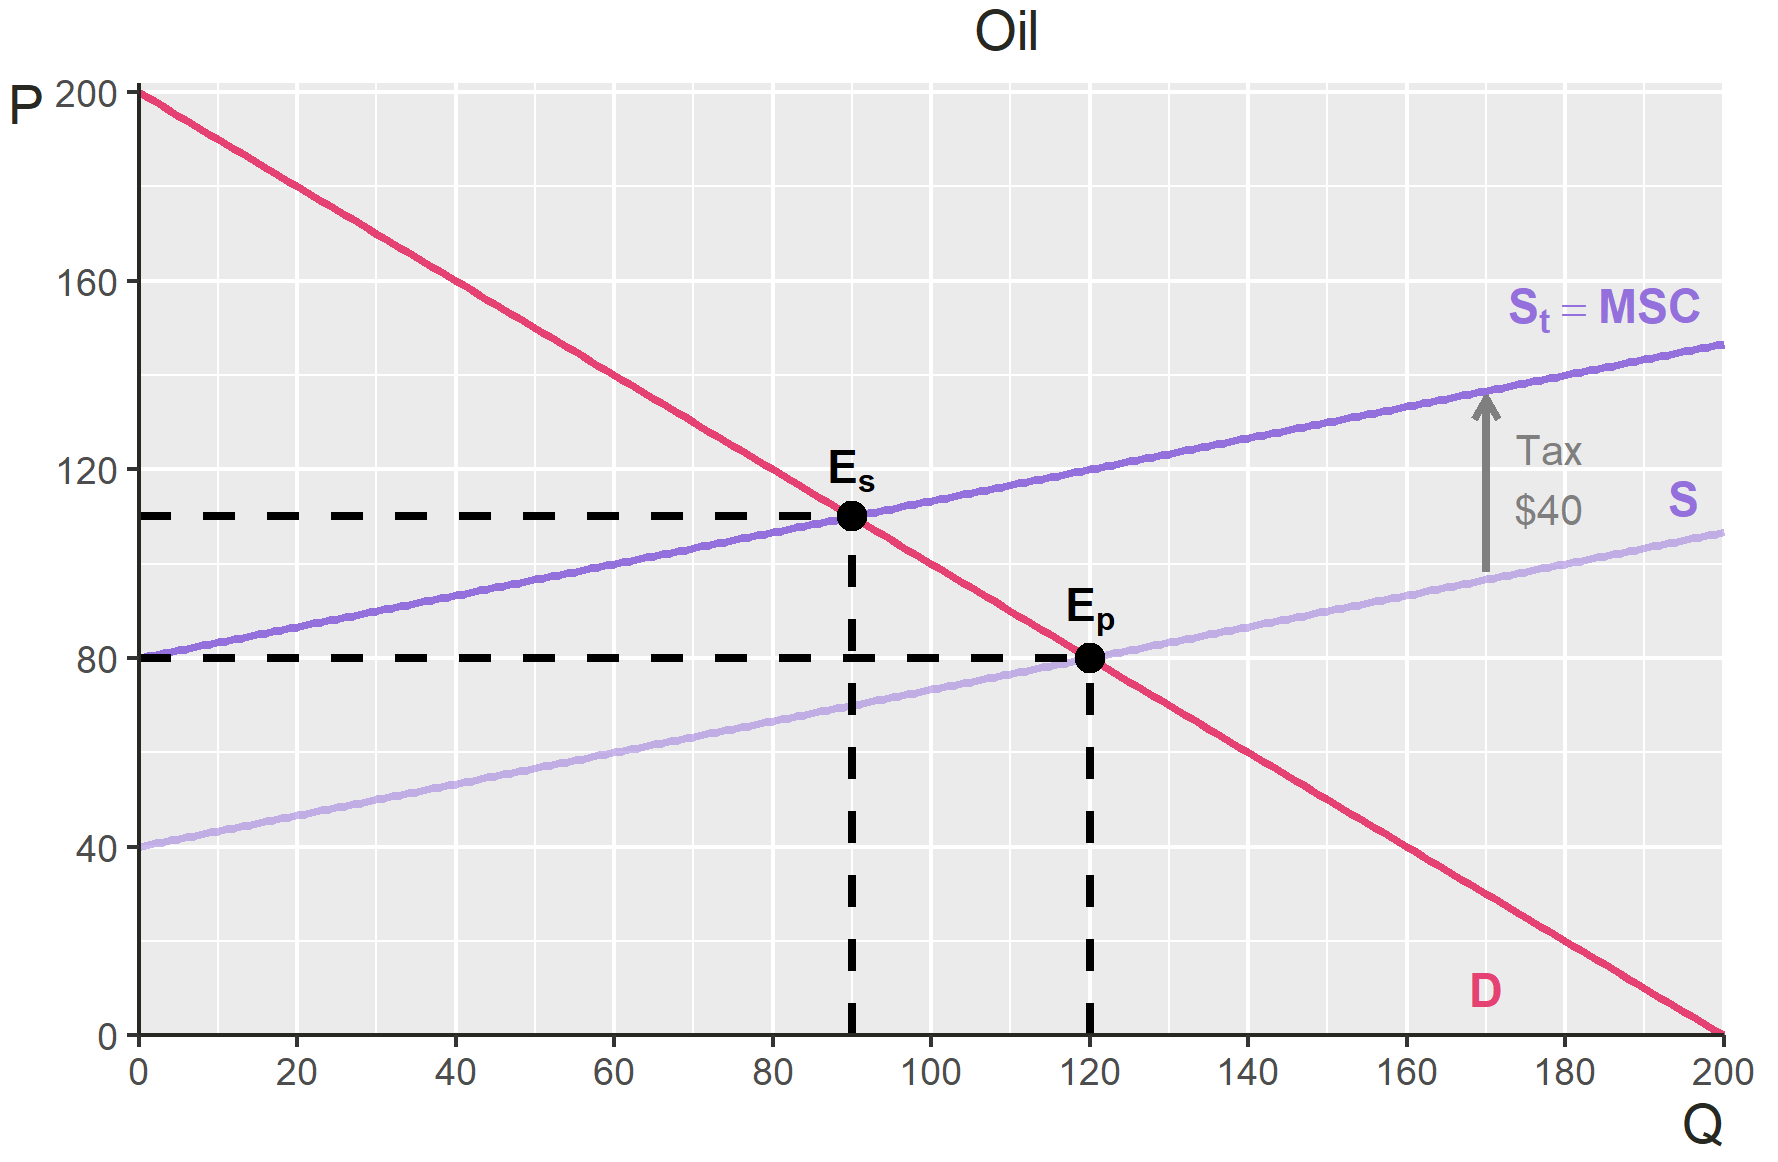
\includegraphics[width=7cm]{pnext tax base.png}
        \end{figure}
    \end{itemize}
\end{frame}

\begin{frame}{Negative Production Externality}
    \begin{itemize}[<+->]
        \item CS and PS are:
        \begin{figure}
            \centering
            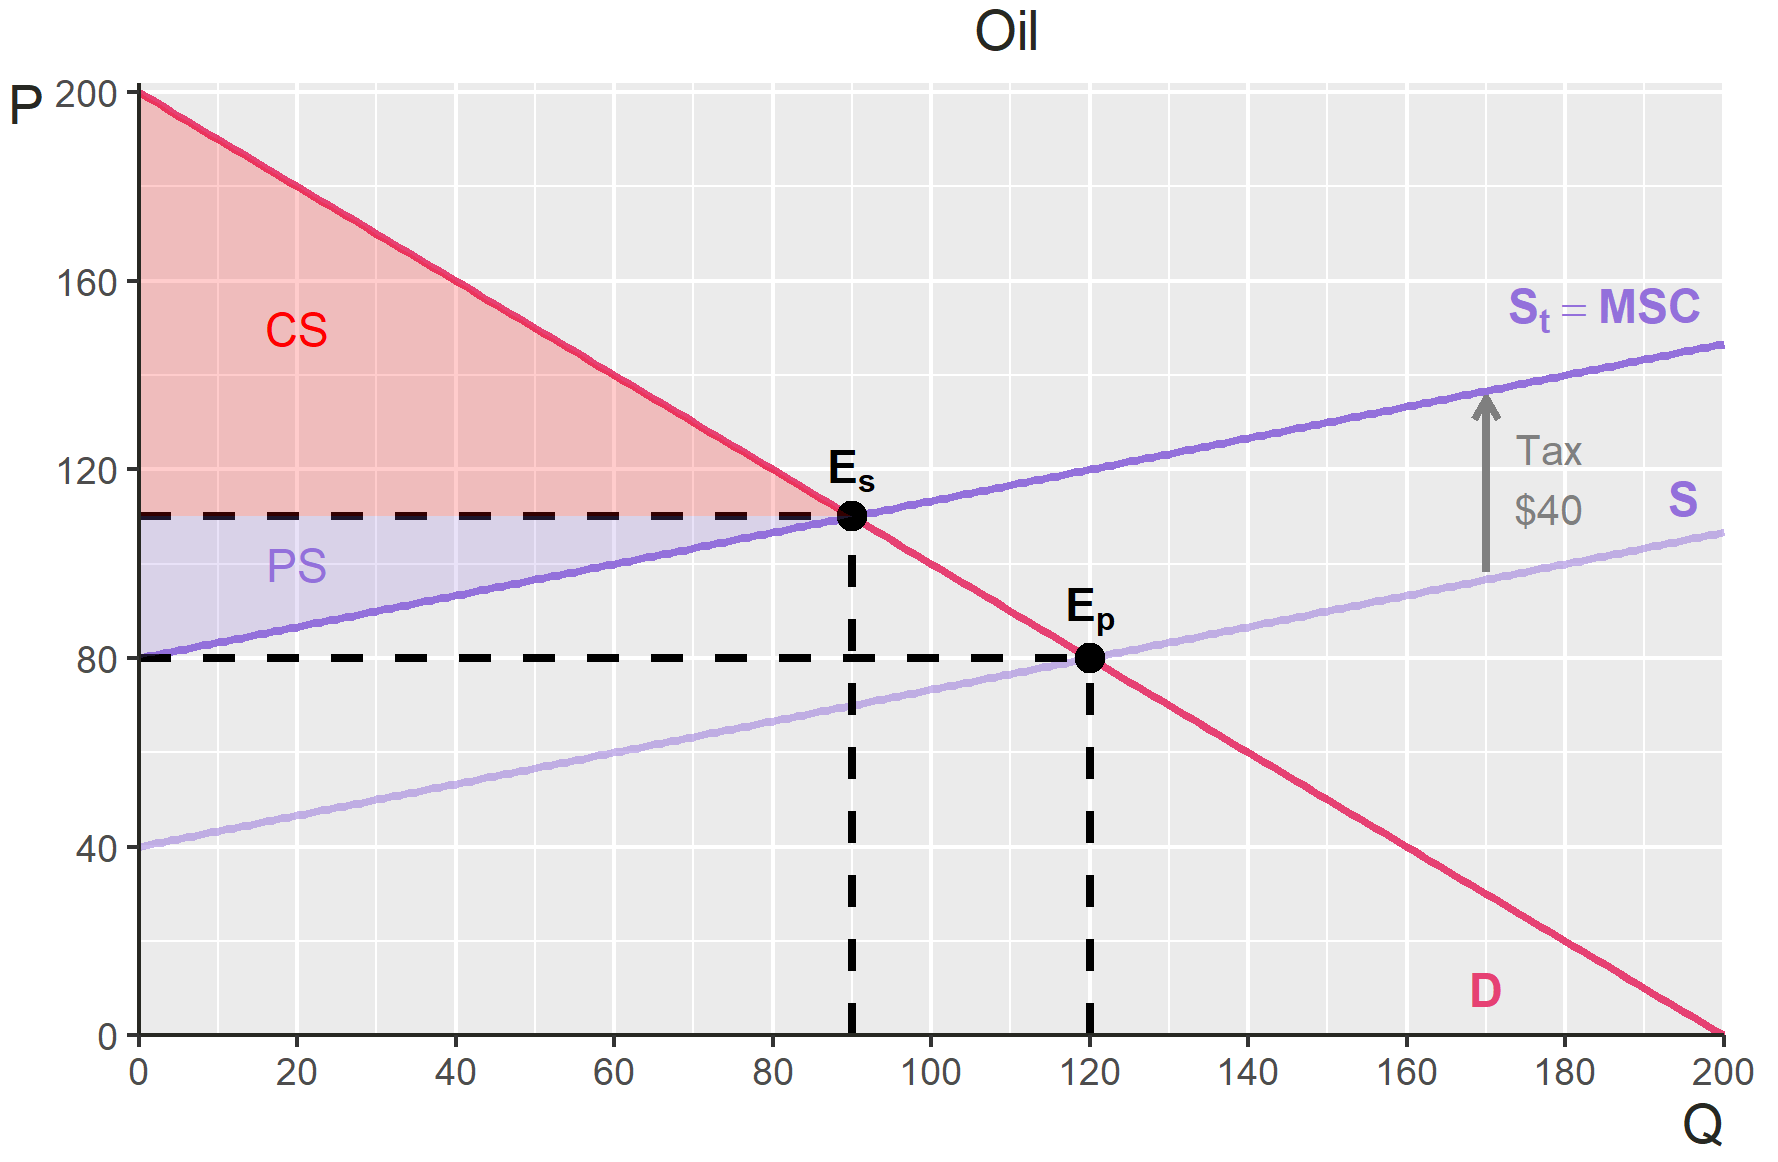
\includegraphics[width=7cm]{pnext tax csps.png}
        \end{figure}
    \end{itemize}
\end{frame}

\begin{frame}{Negative Production Externality}
    \begin{itemize}[<+->]
        \item The EC is now given by
        \begin{figure}
            \centering
            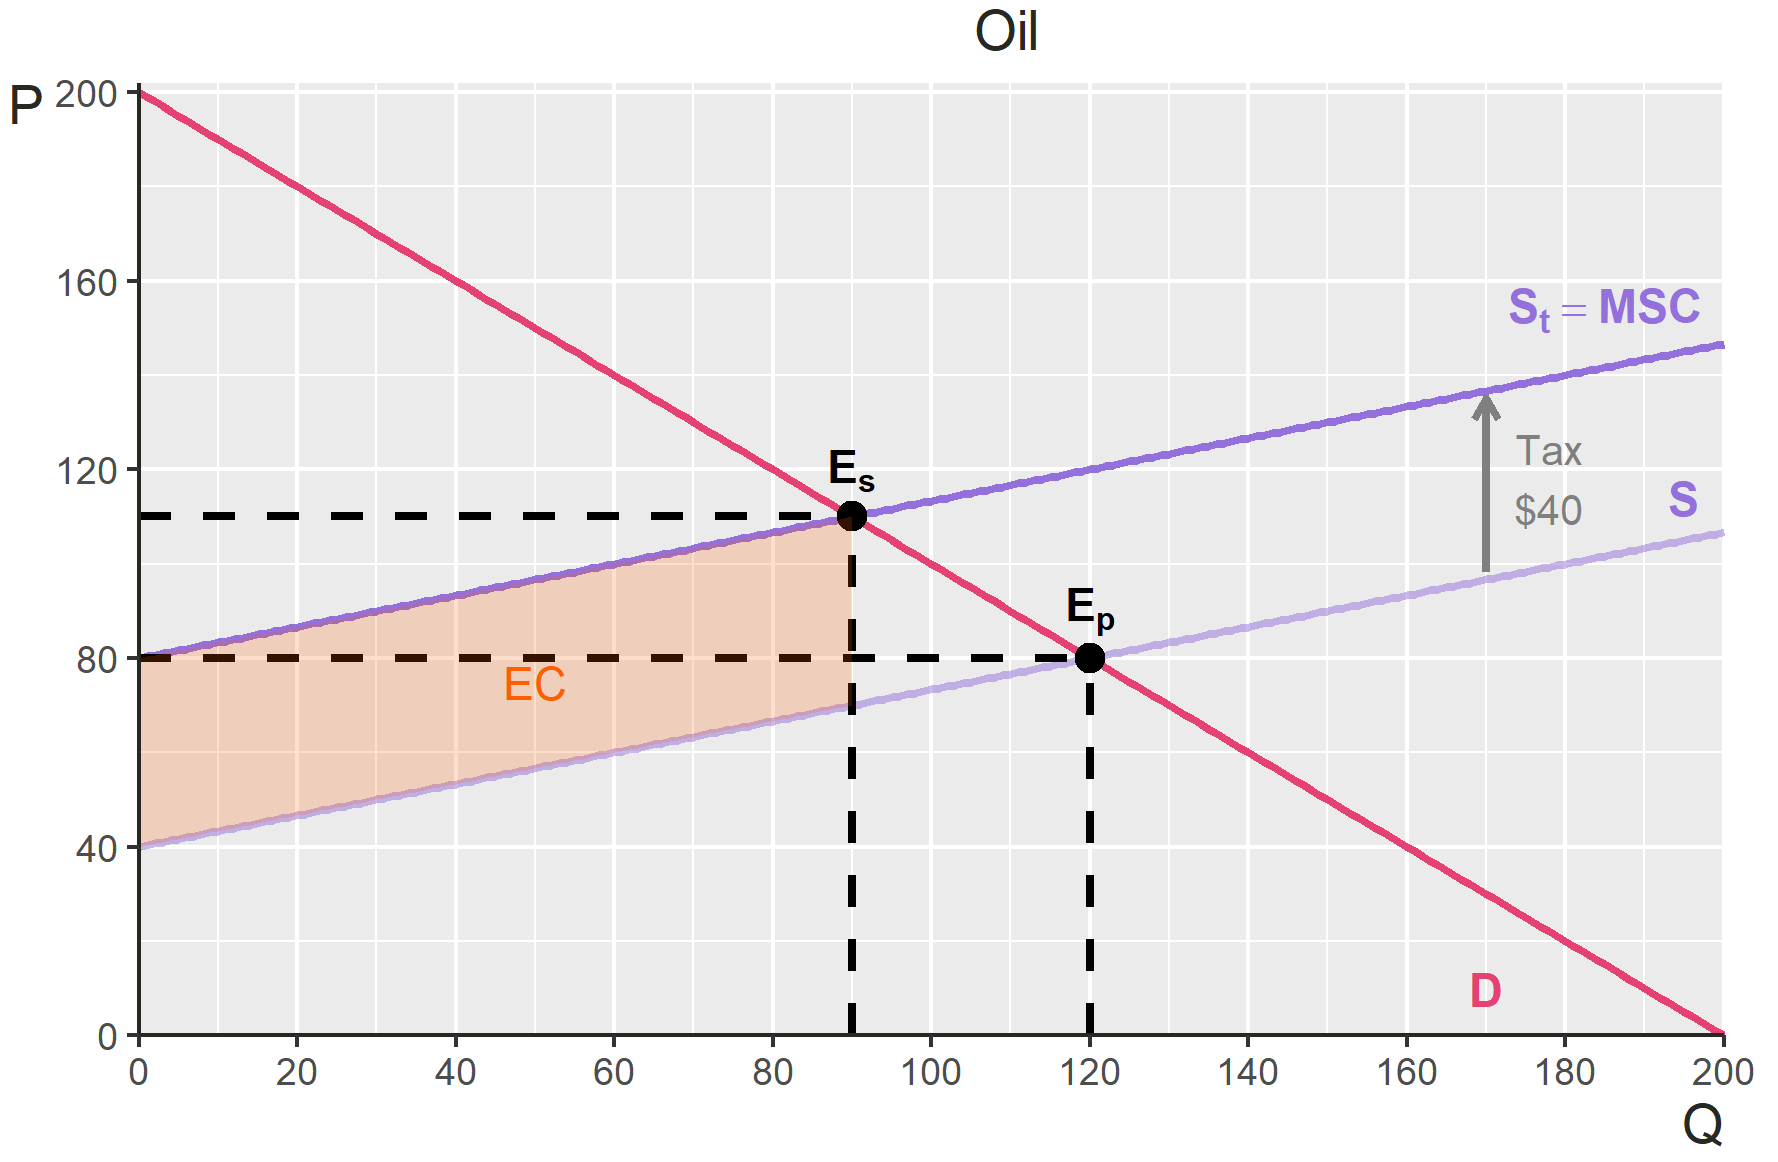
\includegraphics[width=7cm]{pnext tax ec.png}
        \end{figure}
        $$EC=(90)(80-40)=3600$$
    \end{itemize}
\end{frame}

\begin{frame}{Negative Production Externality}
    \begin{itemize}[<+->]
        \item And now, we have some GR
        \begin{figure}
            \centering
            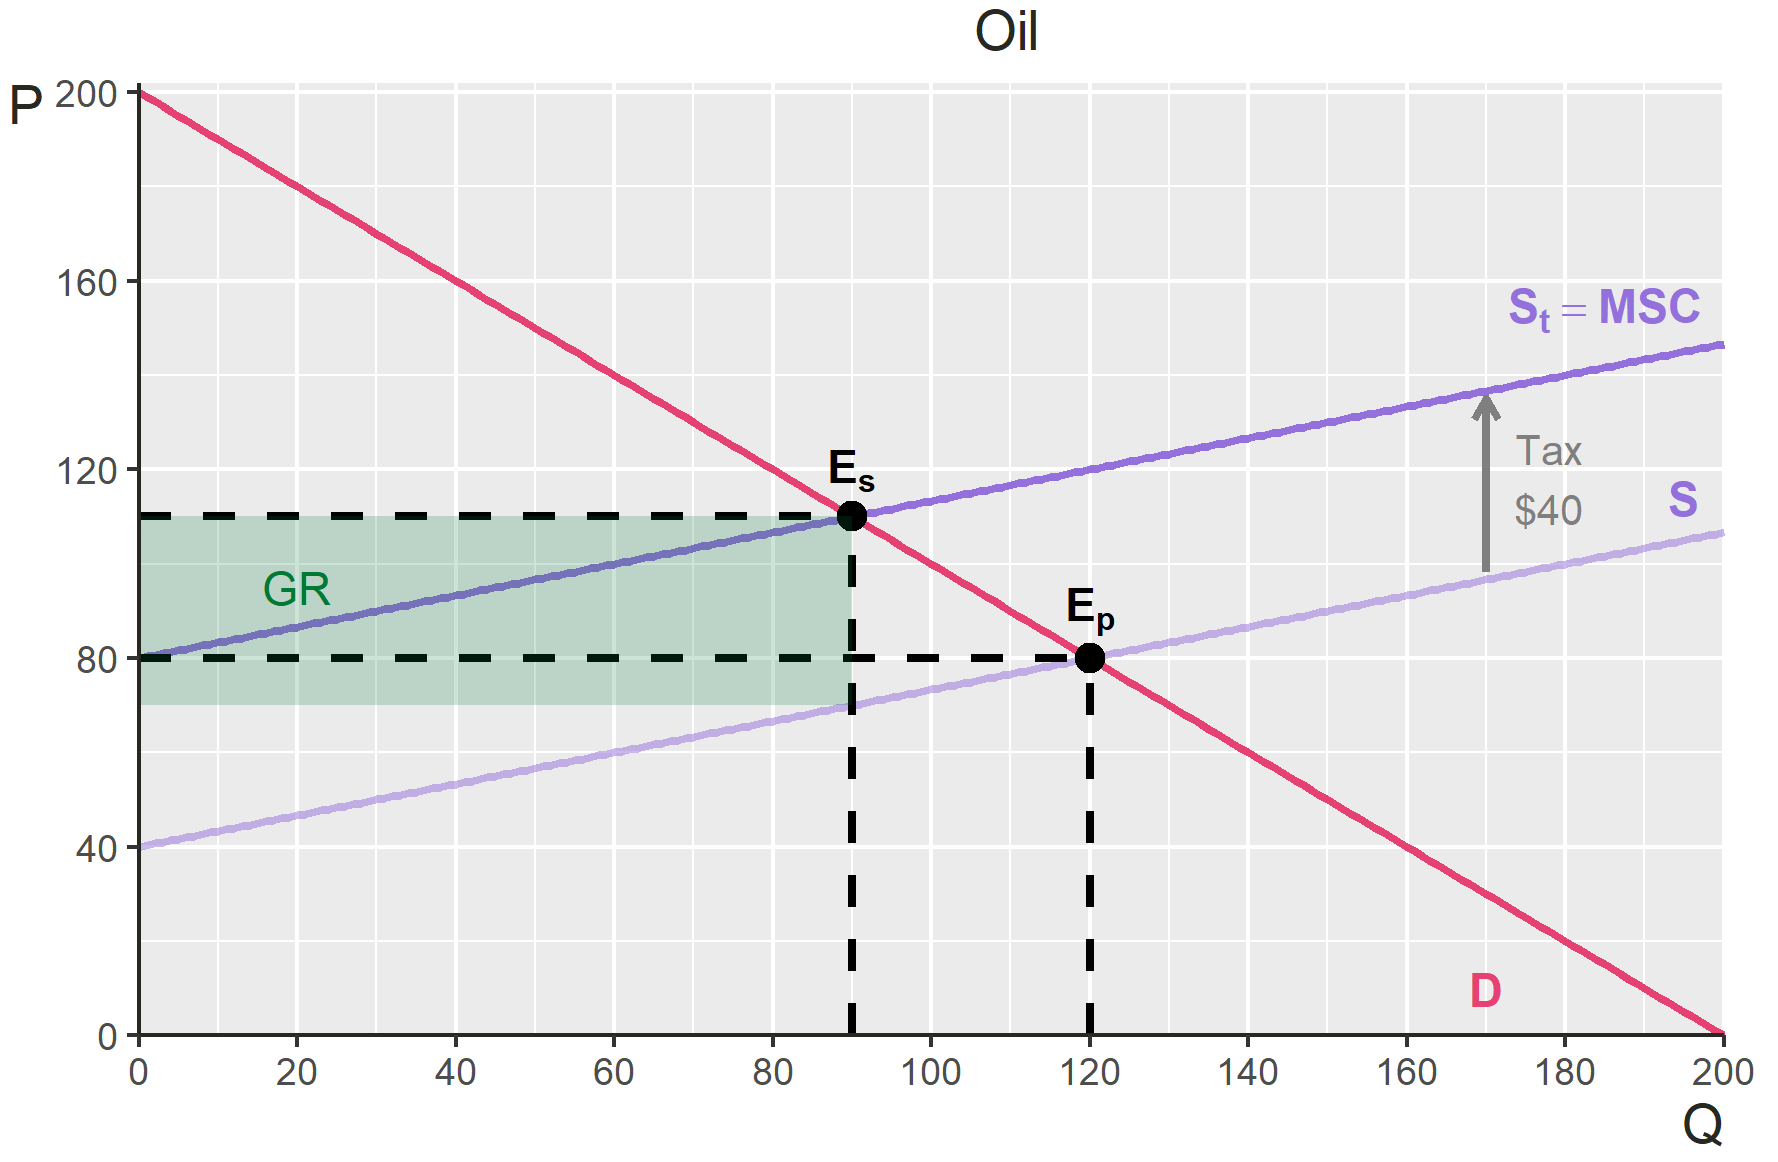
\includegraphics[width=7cm]{pnext tax gr.png}
        \end{figure}
        \item Again, GR exactly cancels out with the new EC
    \end{itemize}
\end{frame}

\begin{frame}{Negative Production Externality}
    \begin{itemize}[<+->]
        \item Therefore, DWL before the tax is given by 
        \begin{figure}
            \centering
            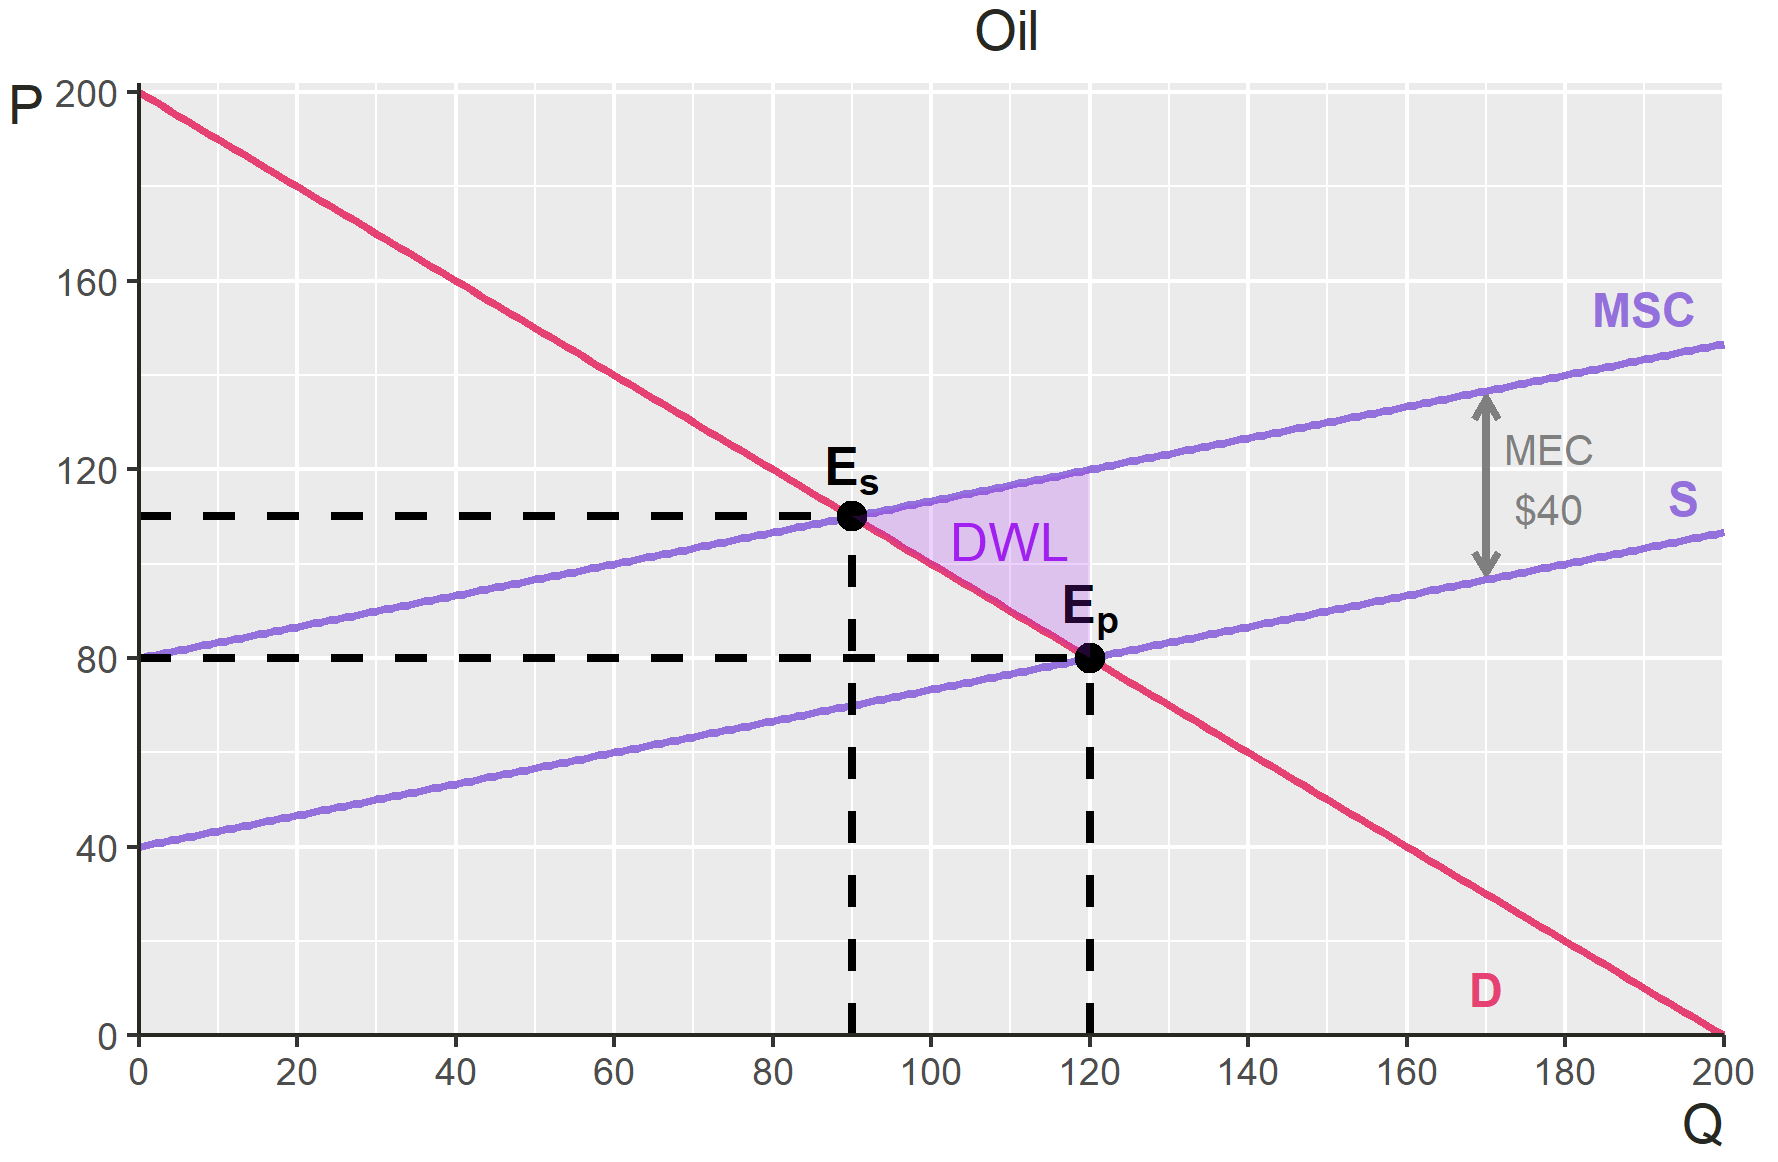
\includegraphics[width=7cm]{pnext dwl.png}
        \end{figure}
        \item I leave it to you to calculate the areas of these figures, and email me with any questions
    \end{itemize}
\end{frame}



%%%%%EX 3
\section*{Positive Externality Example}

\begin{frame}{Positive Consumption Externality}
    \begin{itemize}[<+->]
        \item Consider the market for vegan food, consumed during the entire year (this uses the same numbers as our solar panel example)
        \item Suppose the marginal external benefit, through health expenses and environmental costs, is $\$4000$
        \begin{figure}
            \centering
            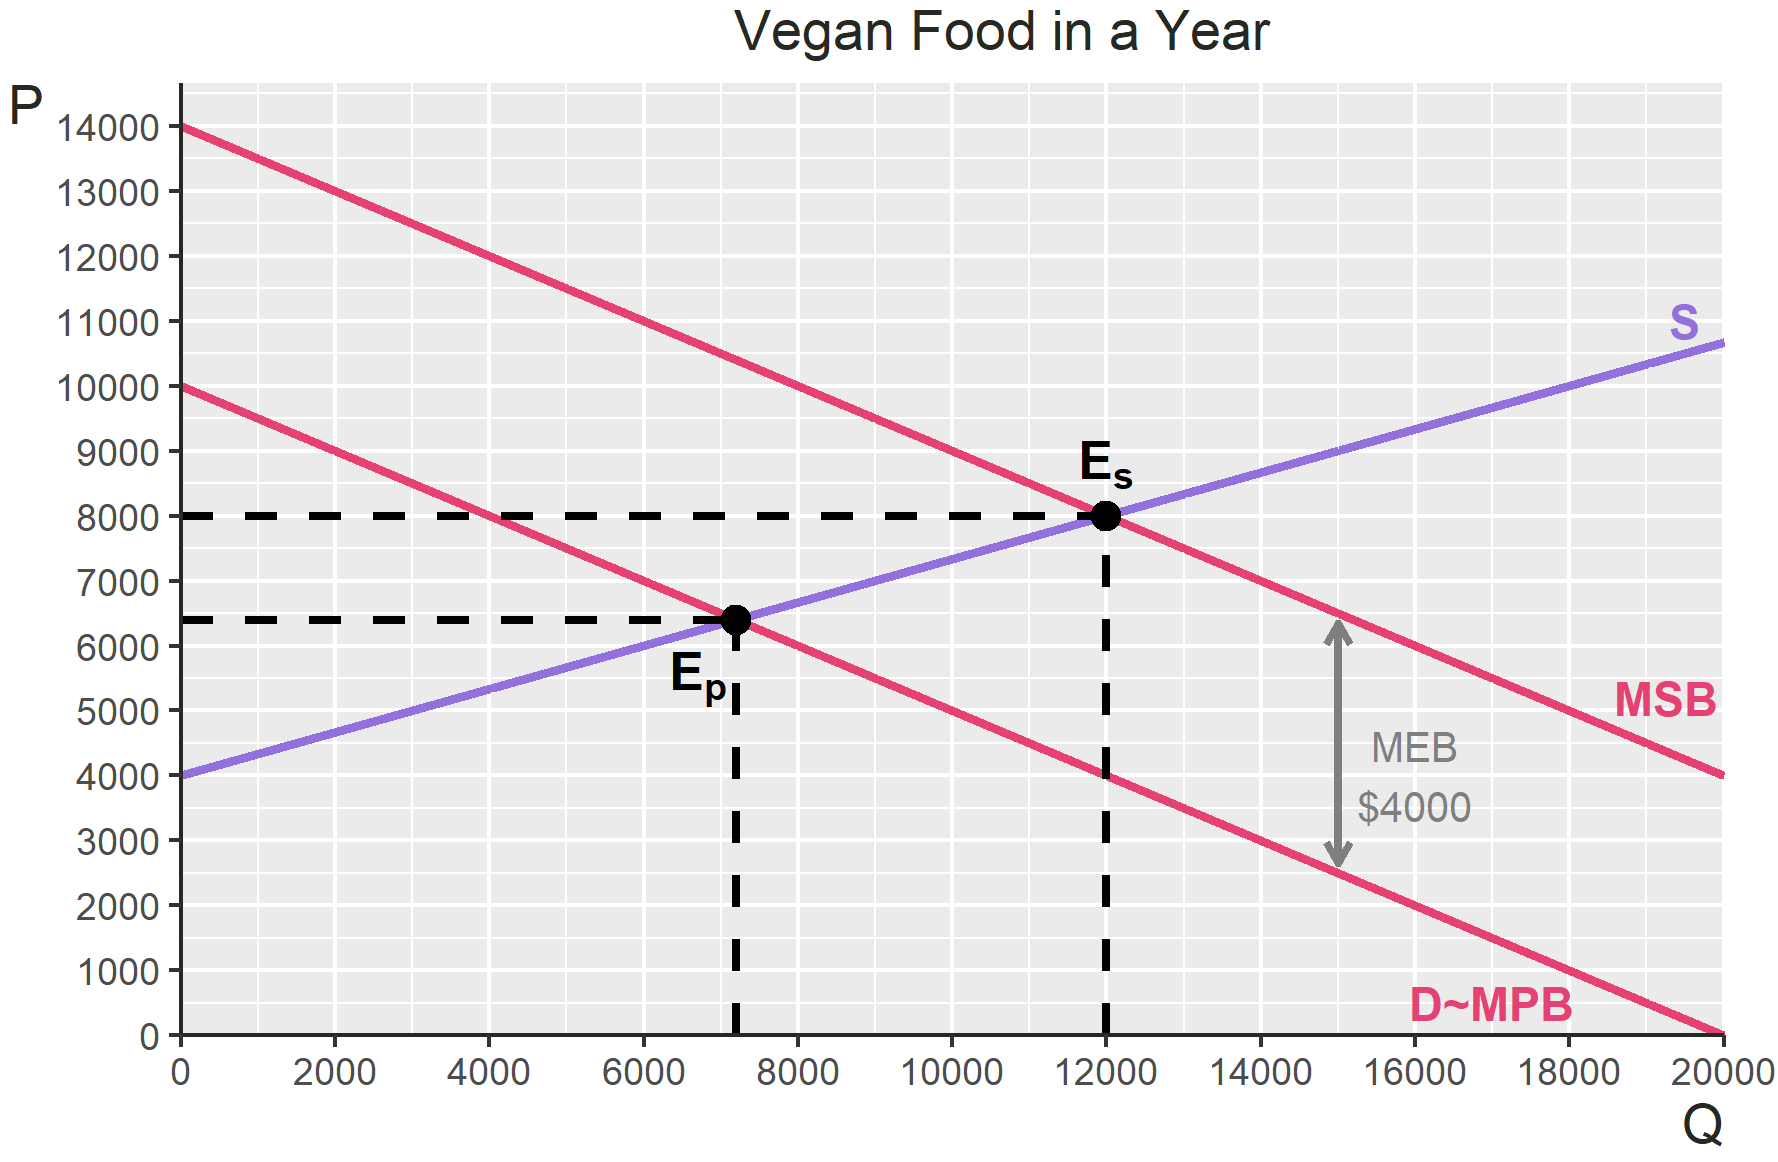
\includegraphics[width=7.5cm]{cpext base.png}
        \end{figure}
    \end{itemize}
\end{frame}

\begin{frame}{Positive Consumption Externality}
        \begin{figure}
            \centering
            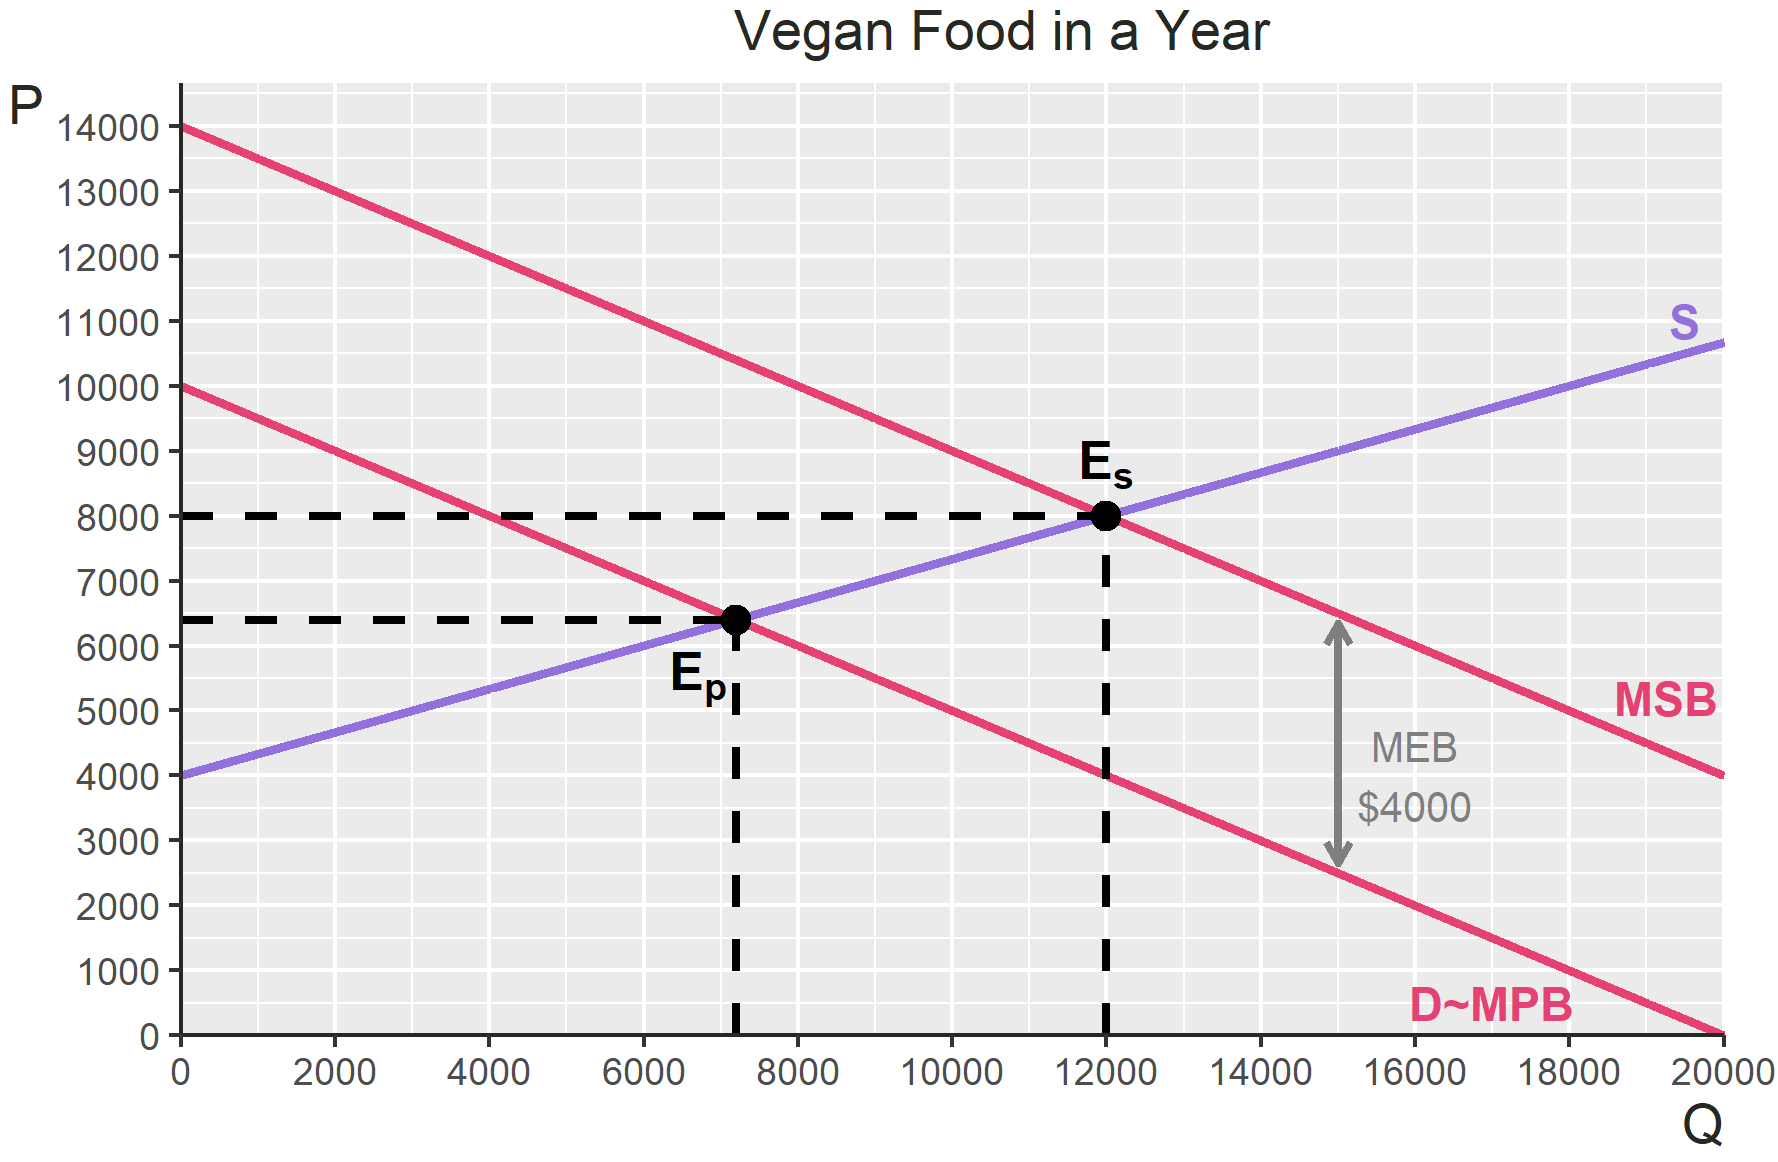
\includegraphics[width=8cm]{cpext base.png}
        \end{figure}
    \begin{itemize}[<+->]
    \vspace{-1mm}
        \item $E_{s}$, how much vegan food society wants to be consumed, due to the benefits, while $E_{p}$ is what happens in reality
    \end{itemize}
\end{frame}


\begin{frame}{Positive Consumption Externality}
    \begin{itemize}[<+->]
    \vspace{-1mm}
        \item What is EB in private equilibrium?
        \begin{figure}
            \centering
            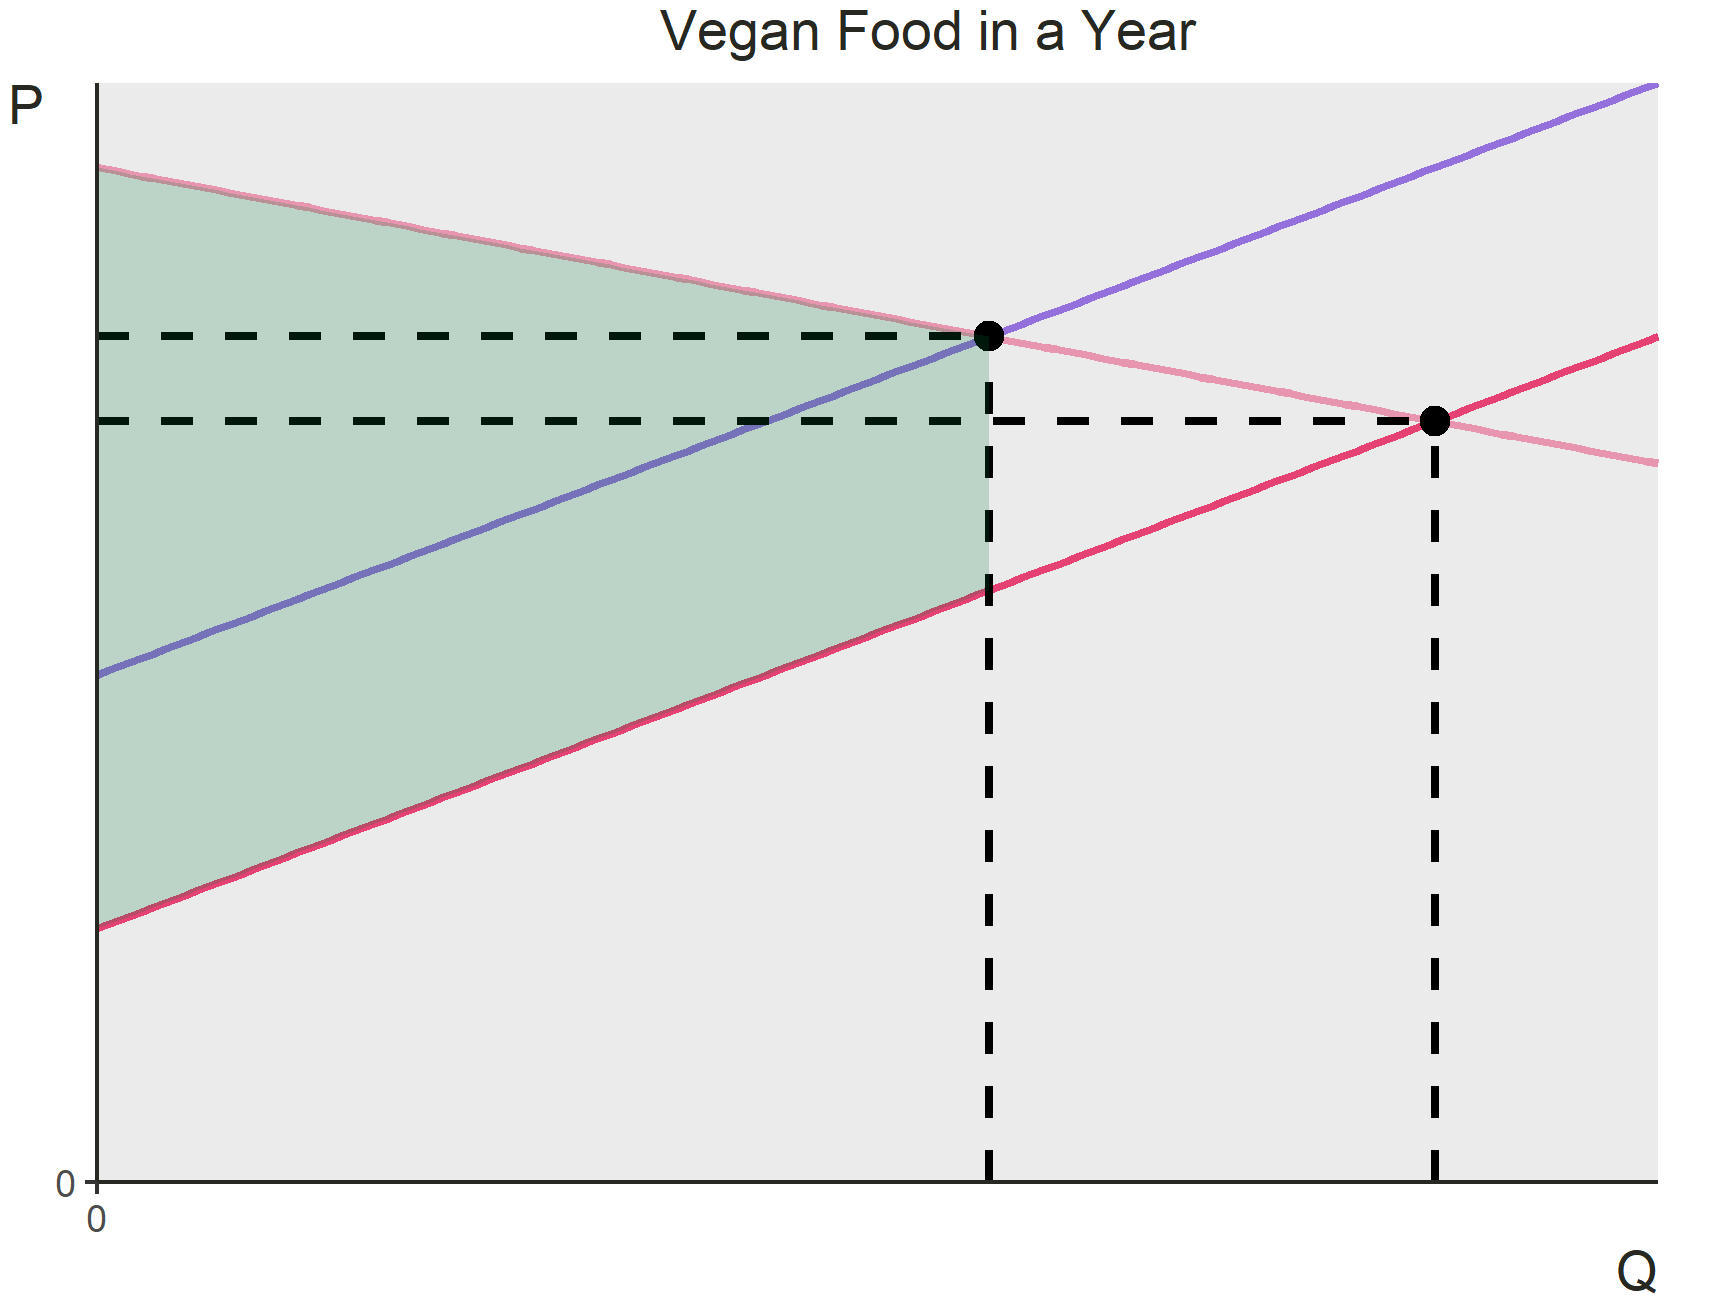
\includegraphics[width=7cm]{cpext eb.png}
        \end{figure}
        $$EB=b\cdot h=7200(14000-10000)=28.8M$$
    \end{itemize}
\end{frame}

\begin{frame}{Positive Consumption Externality}
    \begin{itemize}[<+->]
    \vspace{-1mm}
        \item What is CS+PS in private equilibrium?
        \begin{figure}
            \centering
            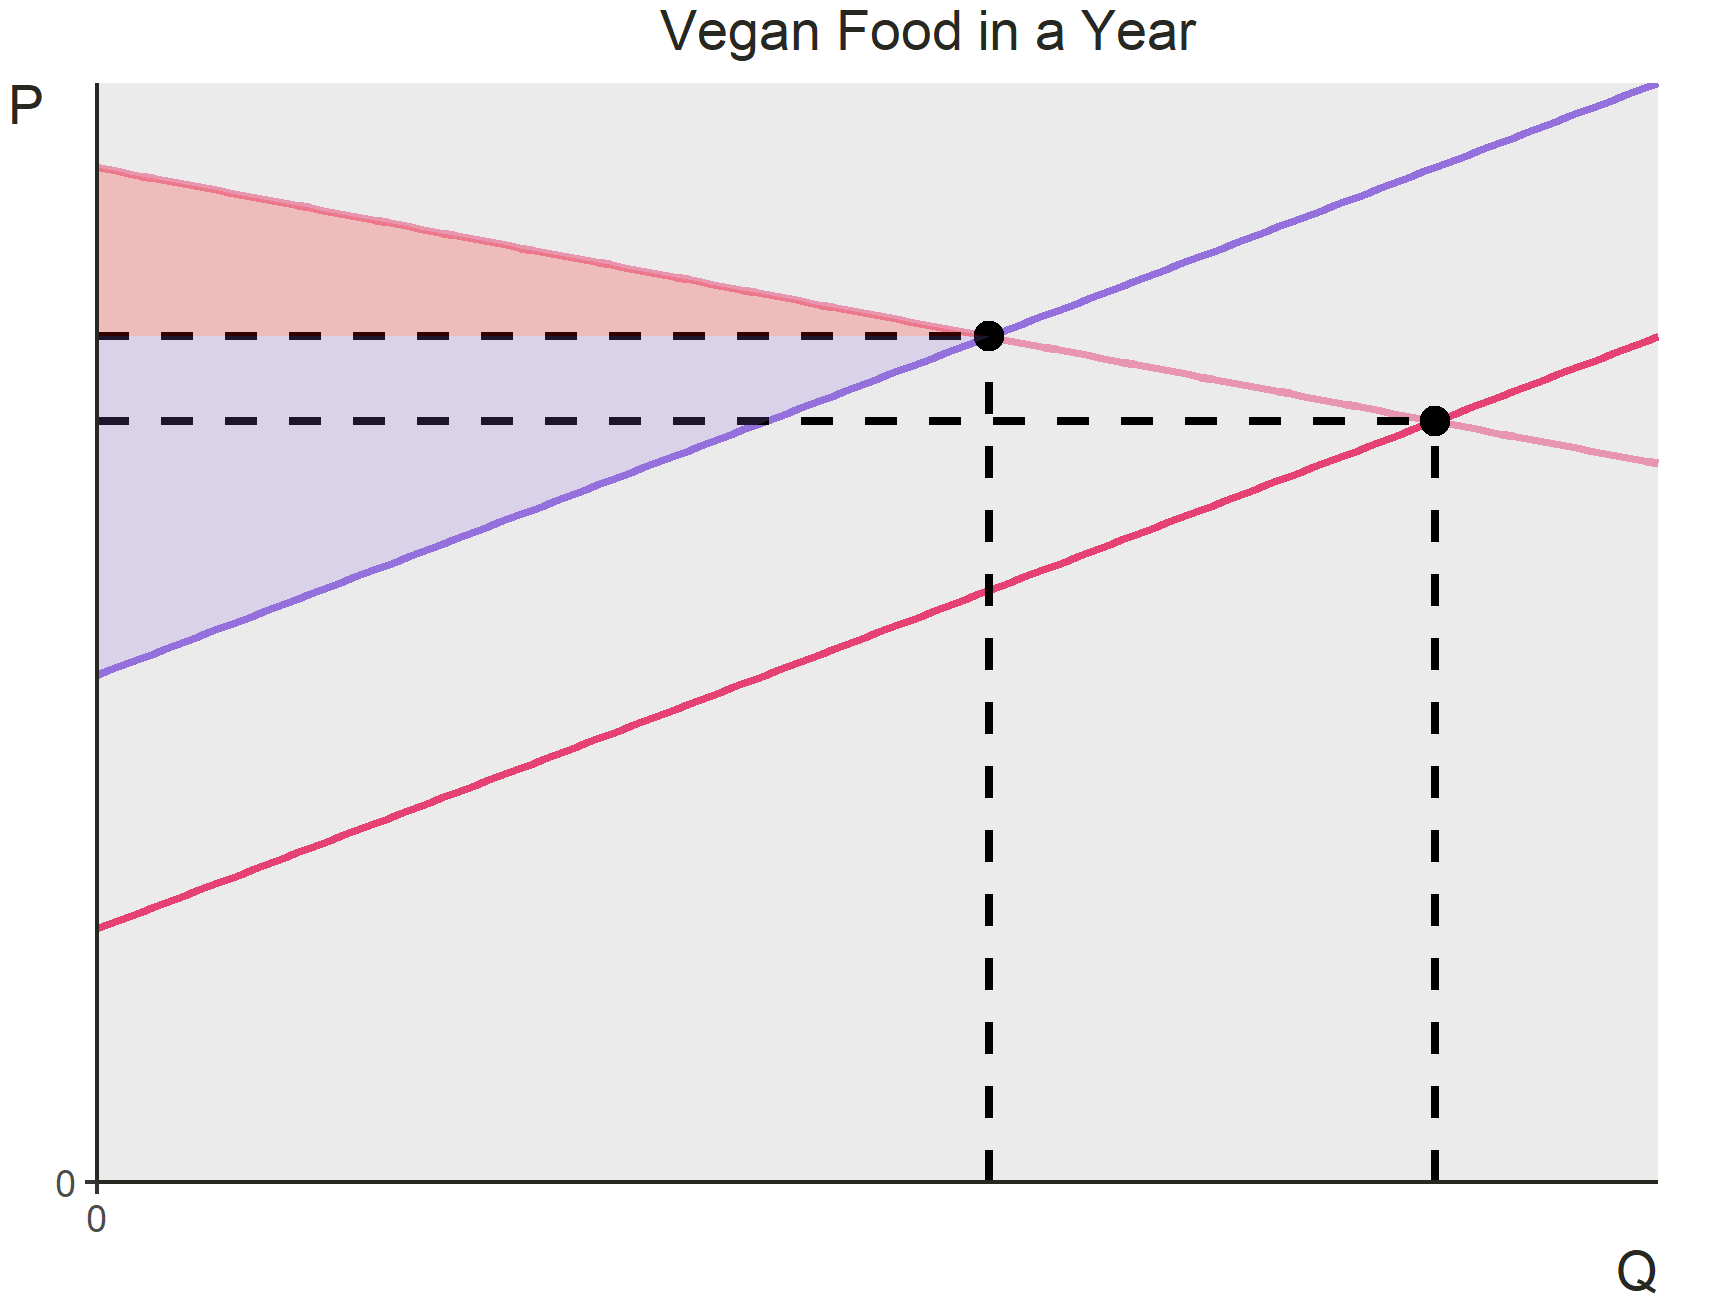
\includegraphics[width=7cm]{cpext csps.png}
        \end{figure}
        \begin{align*}
            CS&=\frac{1}{2}(7200)(10000-6400)=12.96M\\
            PS&=\frac{1}{2}(7200)(6400-4000)=8.64M
        \end{align*}
    \end{itemize}
\end{frame}

\begin{frame}{Positive Consumption Externality}
    \begin{itemize}[<+->]
    \vspace{-1mm}
        \item Thus, total surplus is in private equilibrium is 
        $$TS=CS+PS+EB=12.96M+8.64M+28.8M=50.4M$$
        \item Can we do better?
    \end{itemize}
\end{frame}

\begin{frame}{How do we Correct for Externalities?}
    \begin{itemize}[<+->]
        \item Society benefits when people decide to go vegan. How do we induce someone to go vegan?
        \begin{itemize}
            \item How would you be convinced to go vegan?
            \begin{itemize}
                \item Pay you! 
                \item Pay people to go vegan!
            \end{itemize}
            \item What is this called?
            \begin{itemize}
                \item A subsidy
            \end{itemize}
        \end{itemize}
        \item How much do we pay them?
        \item The exact amount of the marginal external benefit!
    \end{itemize}
\end{frame}

\begin{frame}{Positive Consumption Externality}
    \begin{itemize}[<+->]
        \item With a $\$4000$ subsidy, demand becomes MSB:
        \begin{figure}
            \centering
            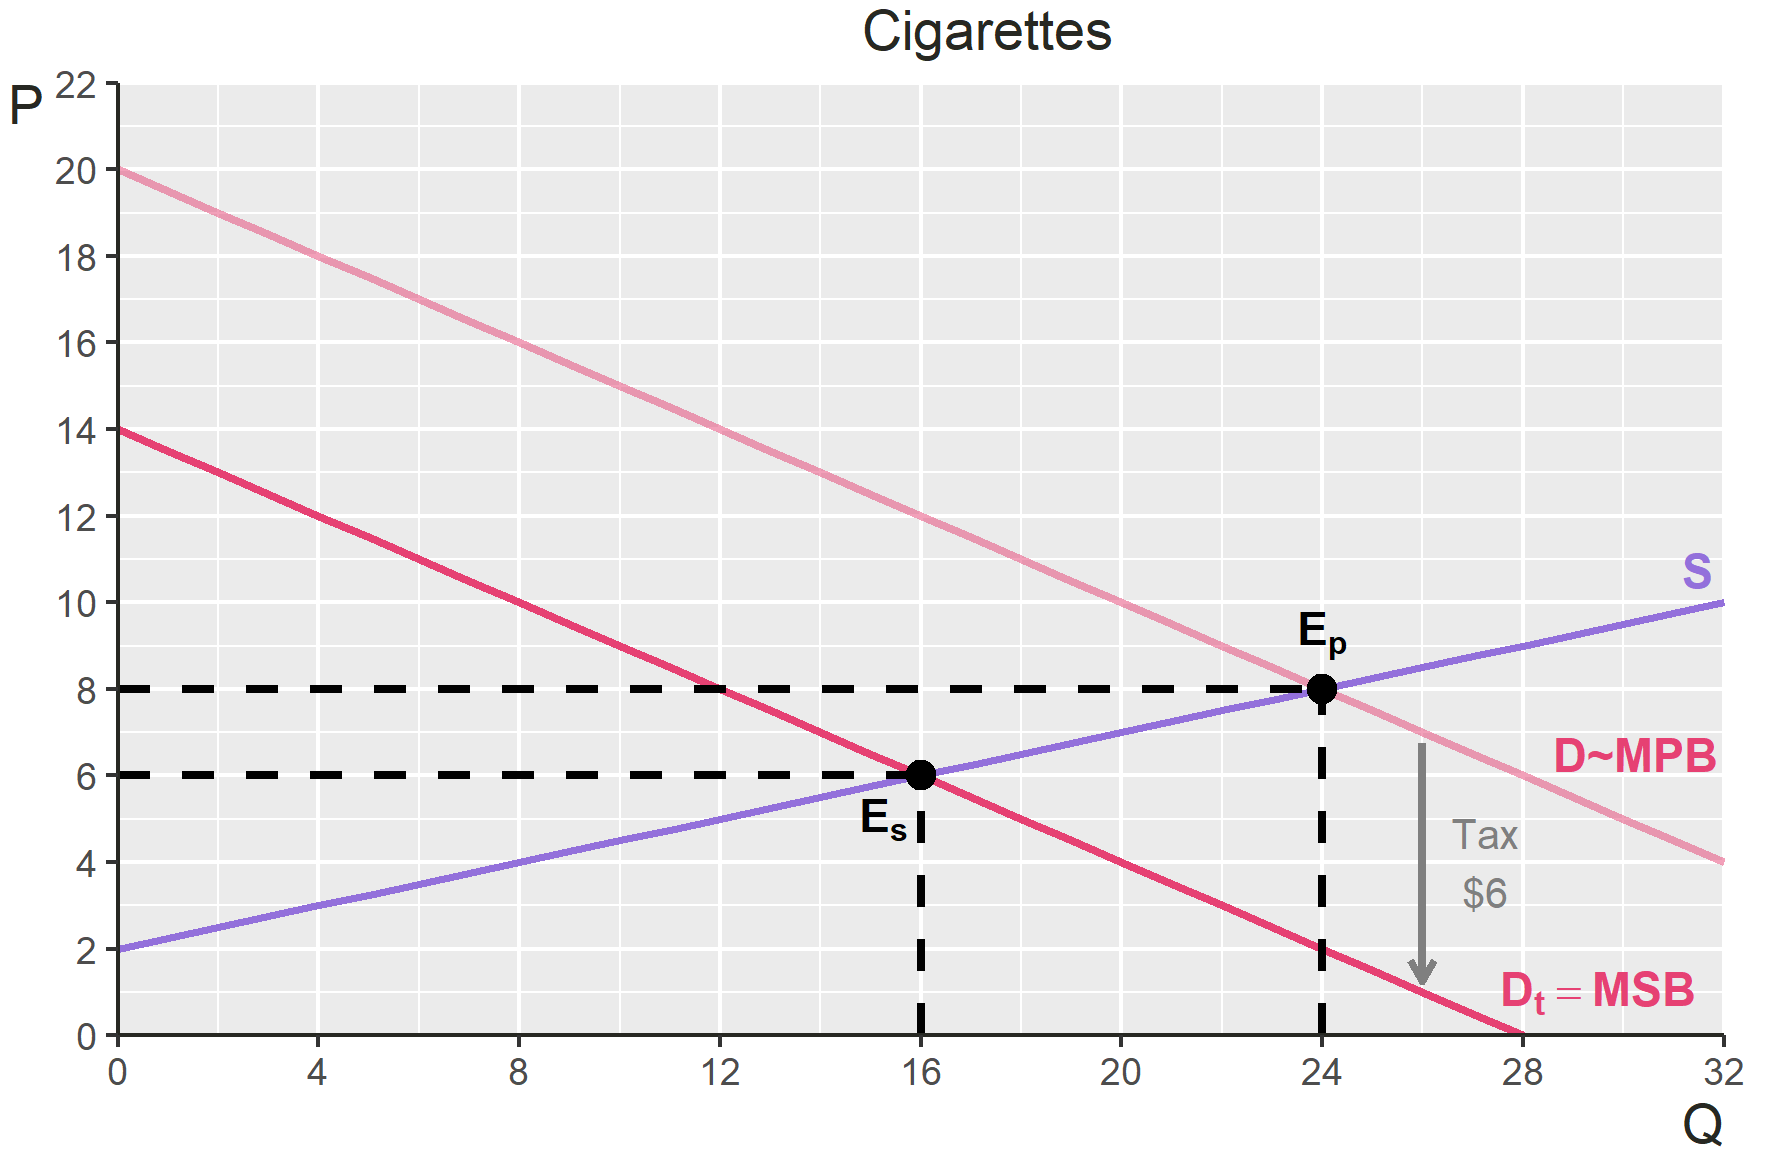
\includegraphics[width=7cm]{cnext tax base.png}
        \end{figure}
    \end{itemize}
\end{frame}

\begin{frame}{Positive Consumption Externality}
    \begin{itemize}[<+->]
        \item CS and PS are as expected:
        \begin{figure}
            \centering
            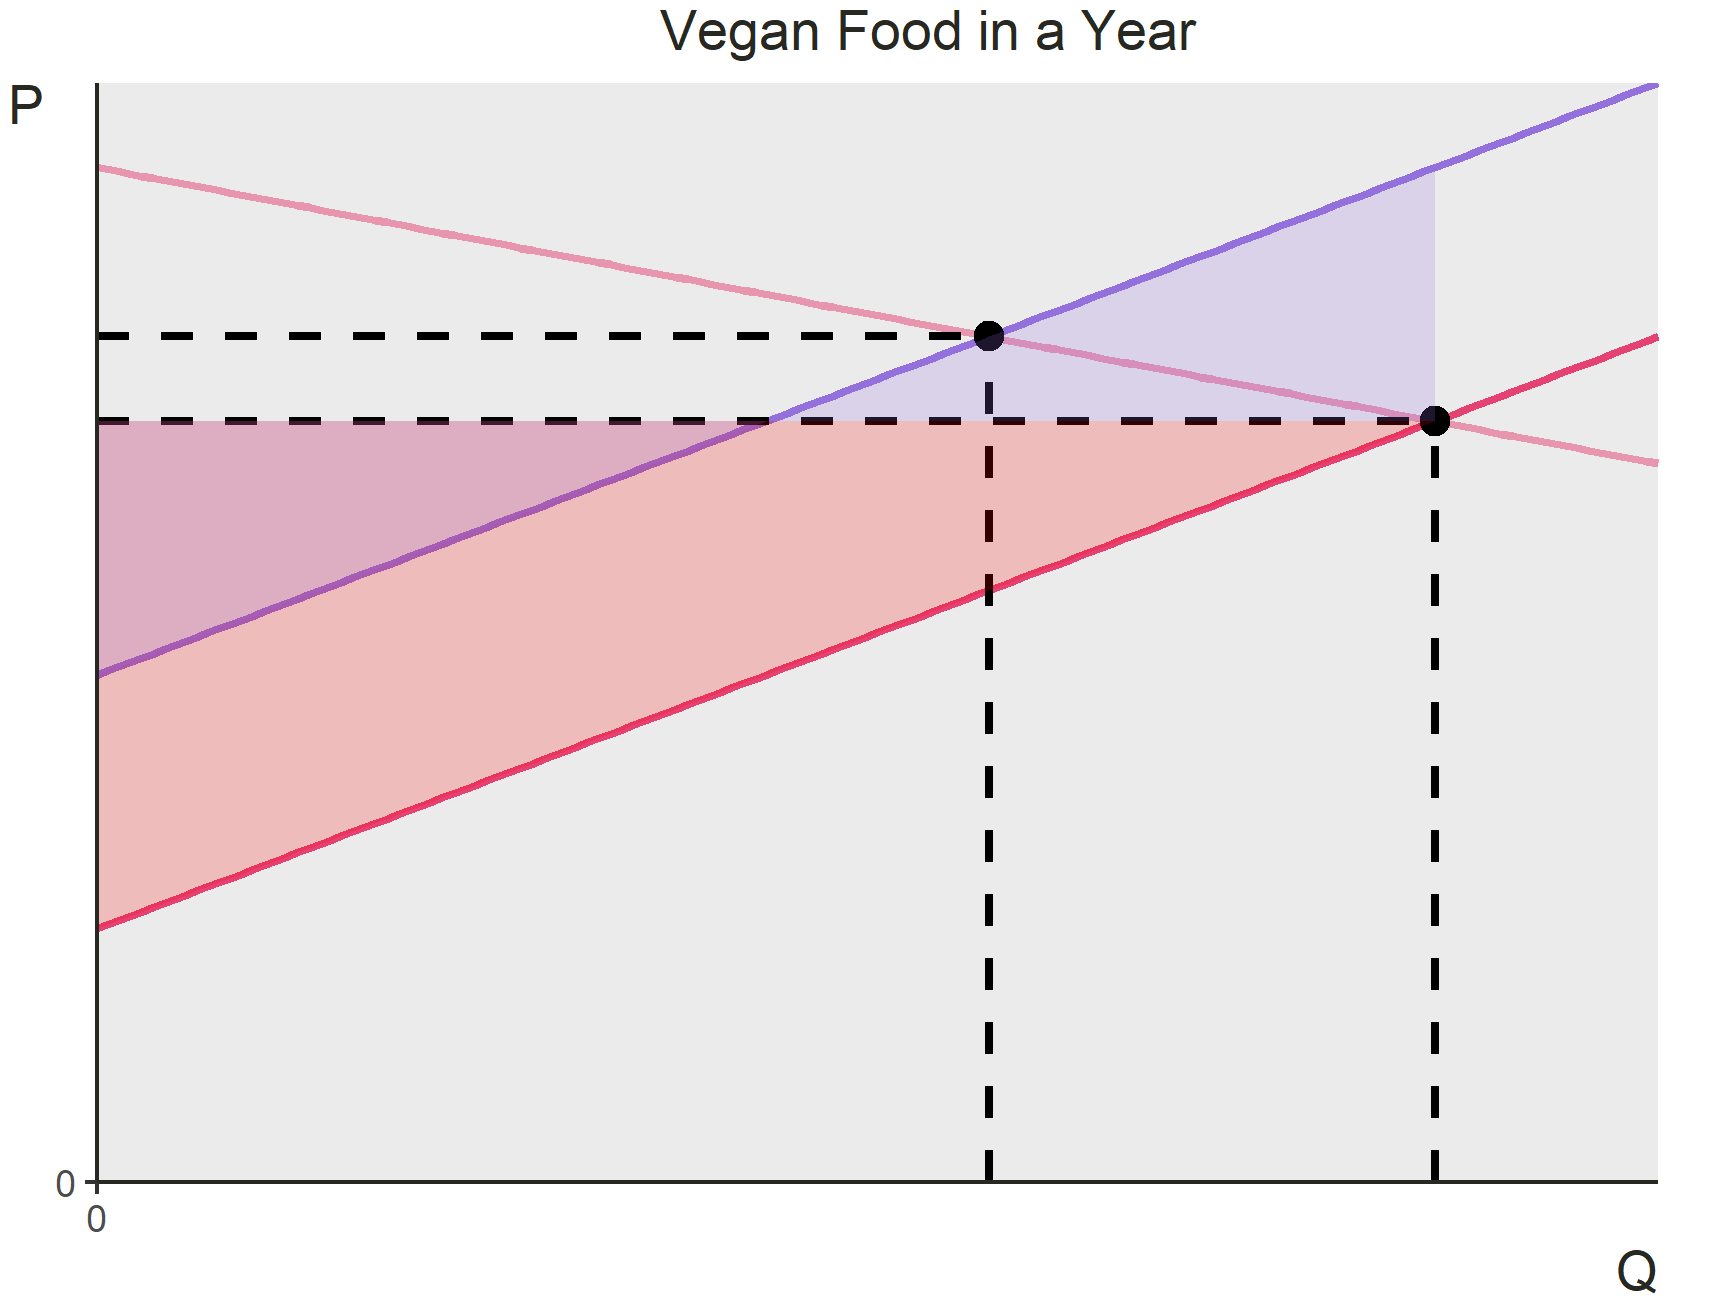
\includegraphics[width=7cm]{cpext tax csps.png}
        \end{figure}
        \begin{align*}
            CS&=\frac{1}{2}(12000)(14000-8000)=36M\\
            PS&=\frac{1}{2}(12000)(8000-4000)=24M
        \end{align*}
    \end{itemize}
\end{frame}

\begin{frame}{Positive Consumption Externality}
    \begin{itemize}[<+->]
        \item The EB is now given by
        \begin{figure}
            \centering
            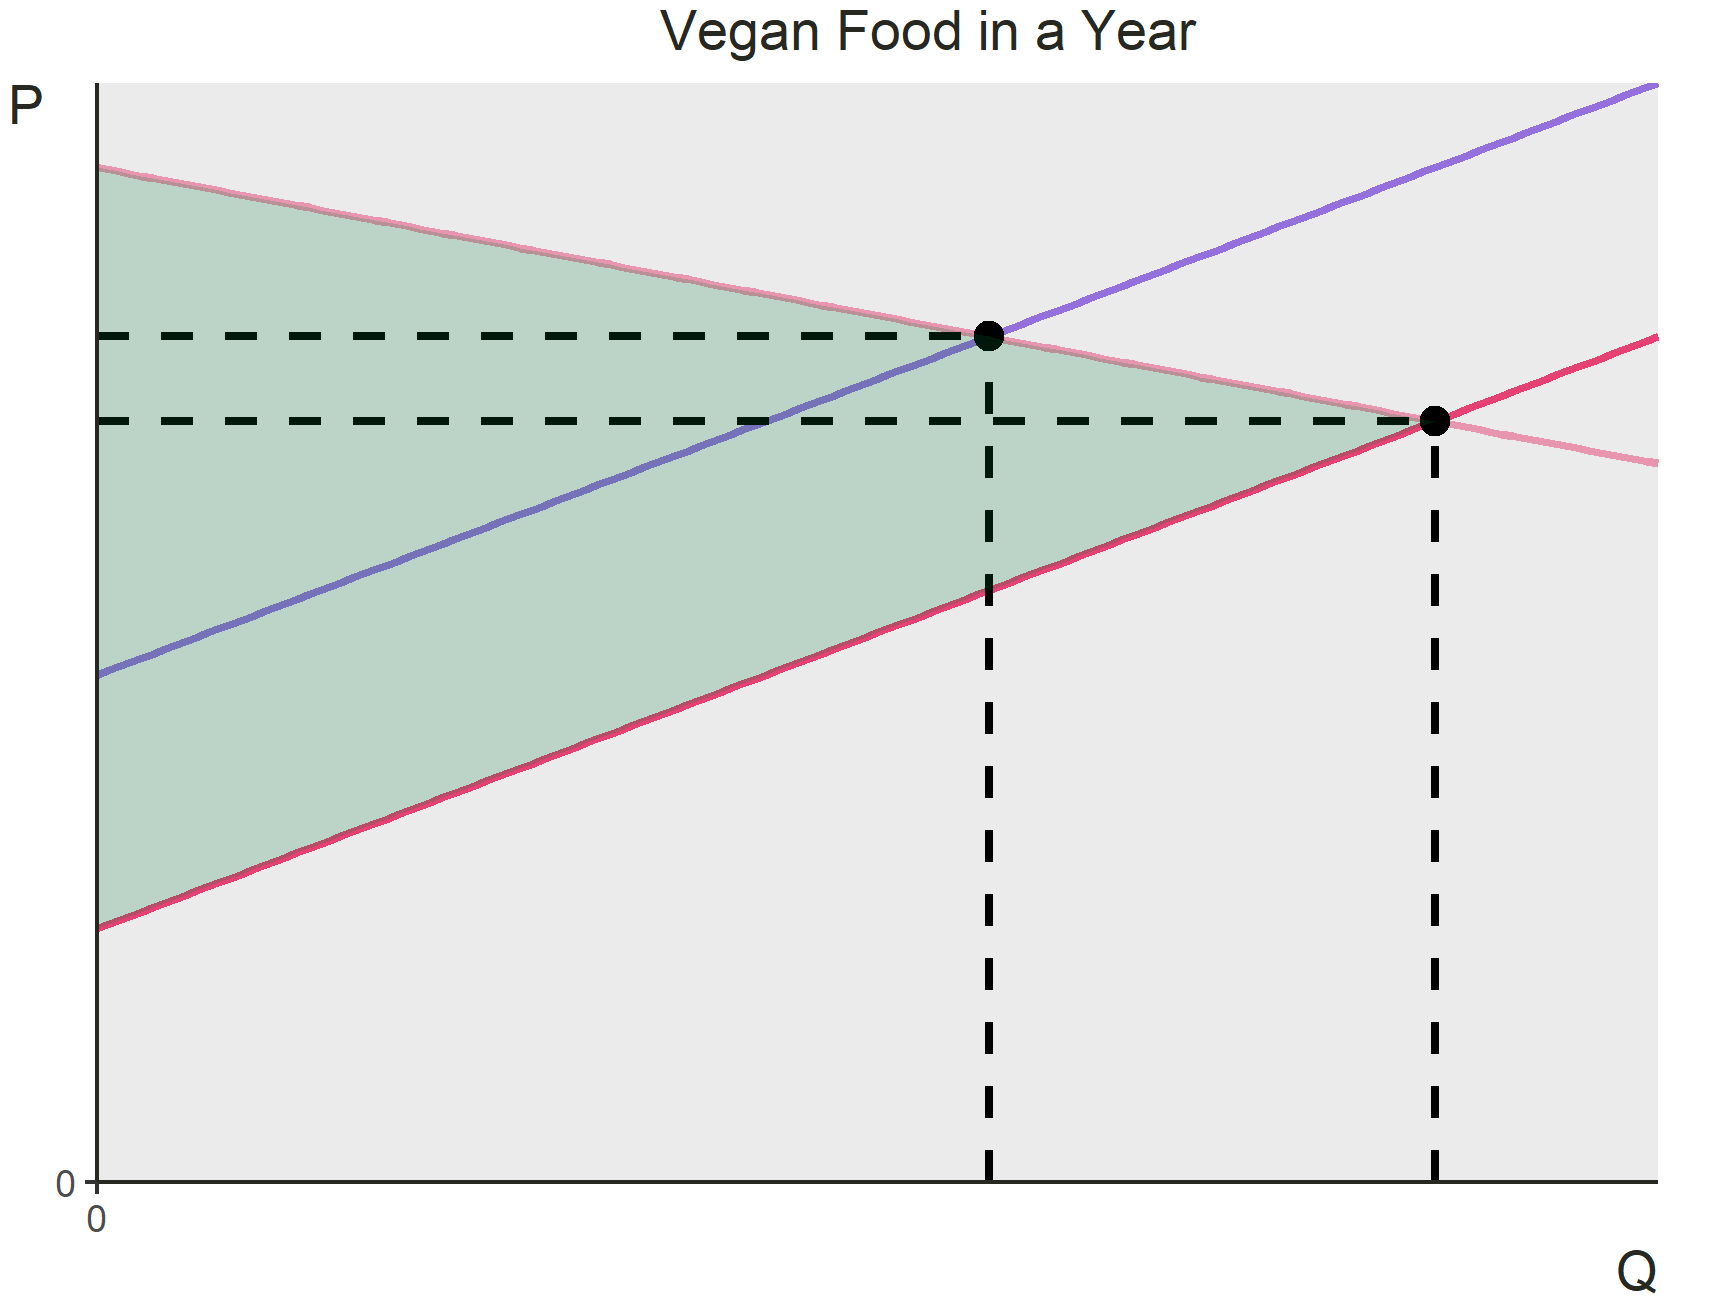
\includegraphics[width=7cm]{cpext tax eb.png}
        \end{figure}
        $$EB=(12000)(14000-10000)=48M$$
    \end{itemize}
\end{frame}

\begin{frame}{Positive Consumption Externality}
    \begin{itemize}[<+->]
        \item And now, we have some GE
        \begin{figure}
            \centering
            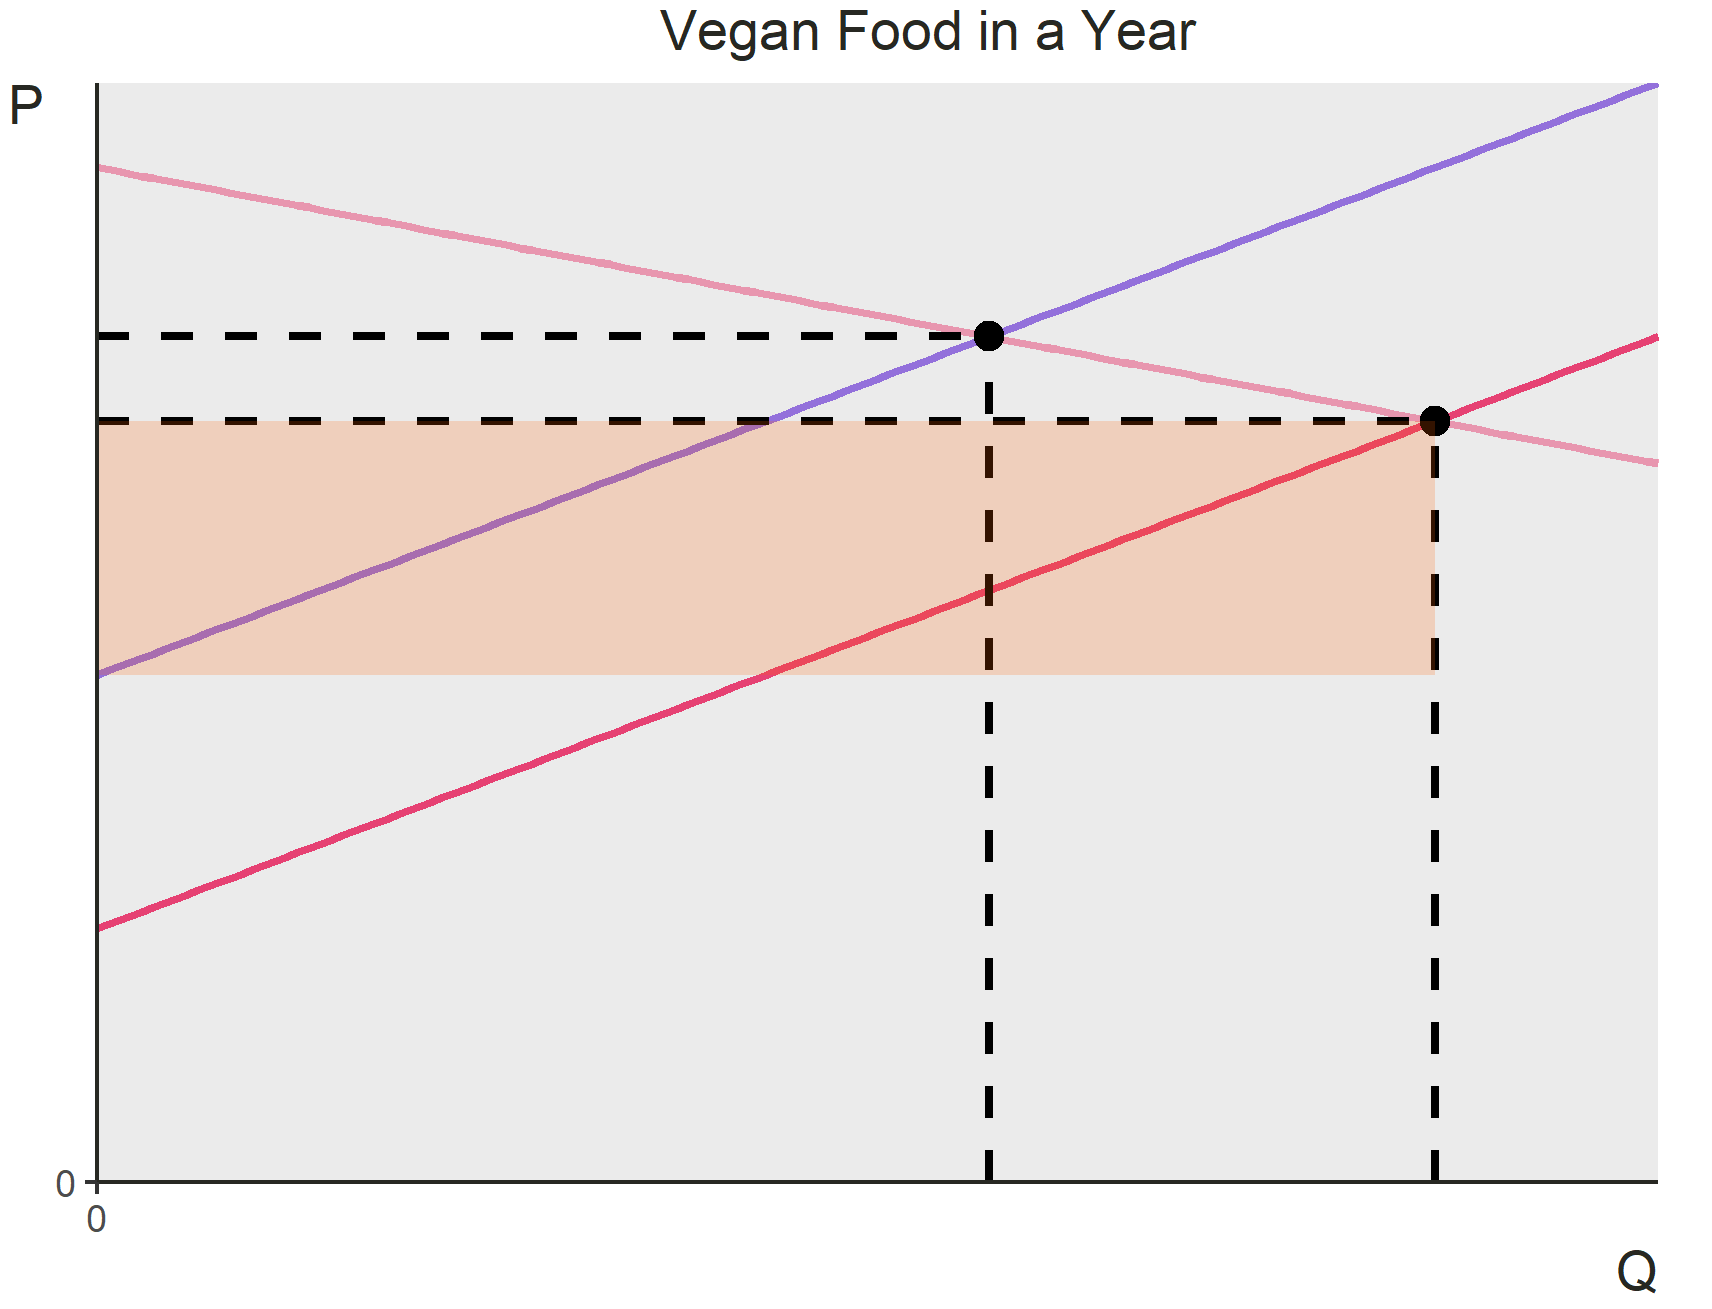
\includegraphics[width=7cm]{cpext tax ge.png}
        \end{figure}
        $$GE=(12000)(8000-4000)=48M$$
    \end{itemize}
\end{frame}

\begin{frame}{Positive Consumption Externality}
    \begin{itemize}[<+->]
        \item As you might expect, GE exactly cancels out with the new EB
        \item What is the new TS?
        \begin{itemize}
            \item The new TS is given by 
            $$TS=CS+PS+EB-GE=36M+24M+48M-48M=60M$$
        \end{itemize}
        \item This beats the $50.4M$ from before, and is in fact the maximum possible TS in this example
        \item Therefore, the subsidy actually \textit{induced} efficiency 
        \begin{itemize}
            \item This is the key lesson: a subsidy will fix a positive externality 
        \end{itemize}
    \end{itemize}
\end{frame}

\begin{frame}{Positive Consumption Externality}
    \begin{itemize}[<+->]
        \item Therefore, DWL before the subsidy is given by 
        \begin{figure}
            \centering
            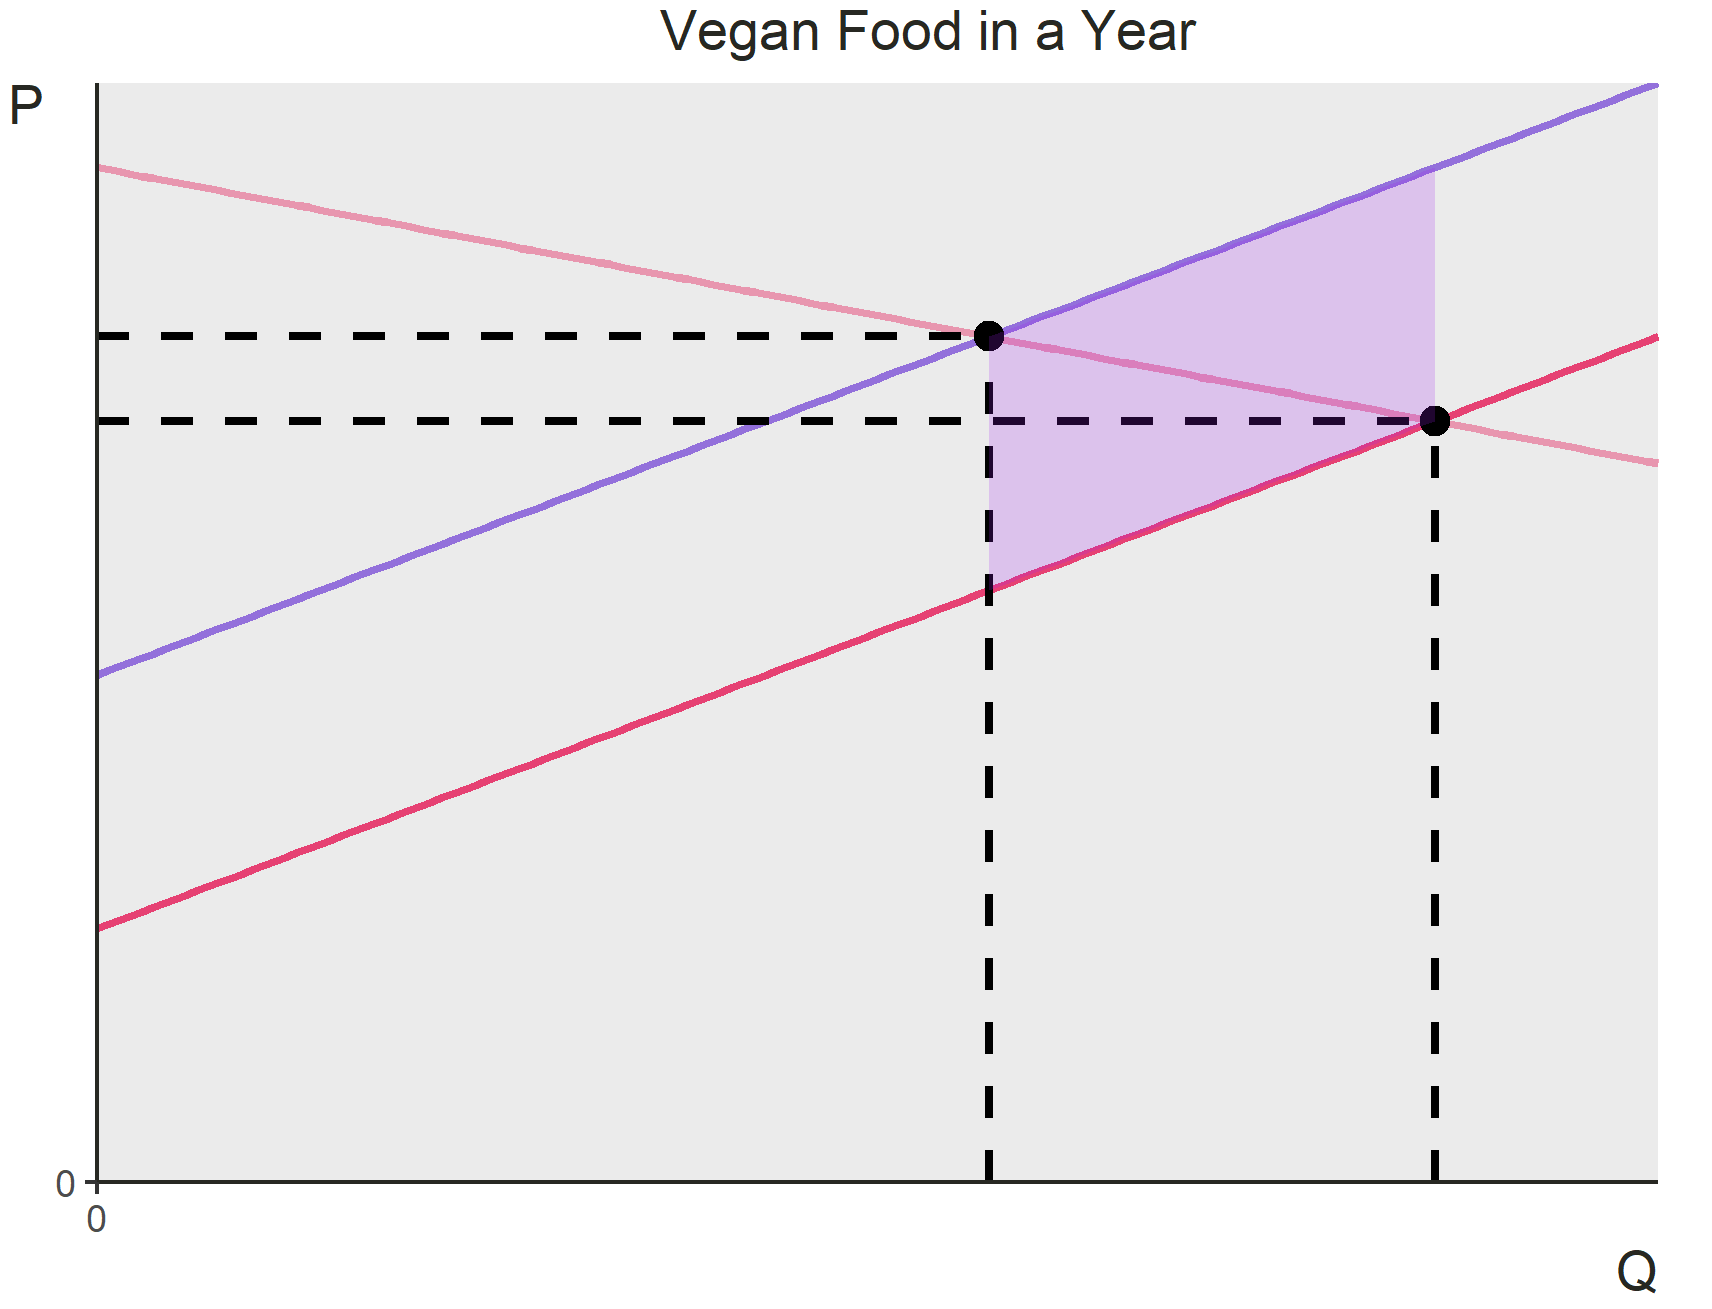
\includegraphics[width=7cm]{cpext dwl.png}
        \end{figure}
        $$DWL=\frac{1}{2}(12000-7200)(8000-4000)=9.6M$$
    \end{itemize}
\end{frame}



\section*{Asides}

\begin{frame}{Aside: Coase Theorem}
    \begin{itemize}[<+->]
        \item If property rights exist, transaction costs are low, and there are few parties involved, then private actors can bargain to eliminate the deadweight loss associated with an externality
        \item Example in homework, if two business are next to each other and one is polluting and ruining the other's business, then the non-polluting firm can pay a little bit to the other firm to produce less
        \item The Coase theorem says that private economic actors can potentially solve the problem of externalities among themselves. Whatever the initial distribution of rights, the interested parties can reach a bargain in which everyone is better off and the outcome is efficient
        \item You may see this here and there, but it is not common enough for me to dive into or test you on; it is just something that is commonly taught
    \end{itemize}
\end{frame}

\begin{frame}{Elasticity and Taxes}
    \begin{itemize}[<+->]
        \item We did not go over what happens to tax mechanisms (burden, surpluses, etc.) when you manipulate elasticity
        \item I may ask you this as a ``new" question on the final
        \item If you want to be prepared for it, and because it is particularly interesting, I would recommend playing around with different slopes and having a fixed tax
        \item I encourage you to try this on your own. If you want some guidance or have questions, you can email me or come to my office hours
        \item This should help you get started for taxes: \href{https://www.desmos.com/calculator/vpcbmkaawa}{Consumer tax and elasticity}, just manipulate $m$ or $s$ (I used $s$, even though it's a tax)
        \item For subsidies, consider these links, which aren't entirely polished (I encourage you to do sketches on your own): 
        \begin{itemize}
        \item \href{https://www.desmos.com/calculator/jh7cvf1iqh}{Subsidy with original fixed point}
        \item \href{https://www.desmos.com/calculator/9mdkivj40d}{Subsidy with new fixed point}
        \end{itemize}
    \end{itemize}
\end{frame}



\end{document}